%% Document class
%\documentclass[12pt,preprint]{aastex}
%\documentclass[preprint2]{aastex}
\documentclass[iop,revtex4]{emulateapj}

%general packages
\usepackage{amsmath}	%for \text{} in math mode
\usepackage{mathrsfs } %for likelihood L
\usepackage{lscape} % landscape environment

%%Figure packages
\usepackage{grffile}	%for dots in filenames
\usepackage{placeins}	%For FloatBarrier

%%Referencinb
\usepackage{hyperref}

%% Custom macros
\newcommand{\vect}[1]{\boldsymbol{#1}} % Uncomment for BOLD vectors.
%\newcommand{\vect}[1]{\vec{#1}} % Uncomment for ARROW vectors.
\newcommand*\diff{\mathop{}\!\mathrm{d}}
\newcommand*\Diff[1]{\mathop{}\!\mathrm{d^#1}}
\newcommand{\pdf}{\ensuremath{pdf}}
\newcommand{\pmodel}{\ensuremath{p_M}}
\newcommand{\MAP}{MAP}
\newcommand{\MAPs}{MAPs}
\newcommand{\RM}{{\sl RoadMapping}}
\makeatletter
\newcommand{\testlabel}[2]{%
   \protected@write \@auxout {}{\string \newlabel {#1}{{#2}{\thepage}{#2}{#1}{}} }%
   \hypertarget{#1}{#2}
}
\makeatother
\usepackage[usenames,dvipsnames]{xcolor}
\newcommand{\Wilma}[1]{\textcolor{Fuchsia}{#1}}
\newcommand{\HW}[1]{\textcolor{Green}{#1}}
\newcommand{\Jo}[1]{\textcolor{Blue}{#1}}

%% Abbreviations
\shorttitle{Action-based Dynamical Models for the Milky Way}
\shortauthors{Trick et al.}

\begin{document}

%% Title [TO DO: Decide on one of them]
%\title{The {\sc RoadMapping} Code:\\How to deal with ``Real World'' Issues\\in Action-based Dynamical Modelling the Milky Way\\}
\title{Action-based Dynamical Modelling of the Milky Way Disk\\with \emph{RoadMapping}\\and our Imperfect Knowledge of the ``Real World''\\}

%% Authors    
\author{Wilma H. Trick\altaffilmark{1,2},  Jo Bovy\altaffilmark{3}, and Hans-Walter Rix\altaffilmark{1}}
\email{trick@mpia.de}

%% Affiliations
\altaffiltext{1}{Max-Planck-Institut f\"ur Astronomie, K\"onigstuhl 17, D-69117 Heidelberg, Germany}
\altaffiltext{2}{Correspondence should be addressed to trick@mpia.de.}
\altaffiltext{3}{University of Toronto [TO DO: What is Jo's current address???]}


%-----------------------------------------------------------------------------------------------------------------------------------------------------------------------------
% Abstract
\begin{abstract}
We present \RM{}, a dynamical modelling machinery that aims to recover the Milky Way's (MW) gravitational potential and the orbit distribution of stellar populations in the Galactic disk. \RM{} is a full likelihood analysis that models the observed positions and velocities of stars with an equilibrium, three-integral distribution function (DF) in an axisymmetric potential. In preparation for the application to the large data sets of modern surveys like Gaia, we create and analyze a large suite of mock data sets and develop qualitative ``rules of thumb'' for which characteristics and limitations of data, model and machinery affect constraints on the potential and DF most. We find that, while the precision of the recovery increases with the number of stars, the numerical accuracy of the likelihood normalisation becomes increasingly important and dominates the computational efforts. The modelling has to account for the survey's selection function, but \RM{} seems to be very robust against small misjudgments of  the data completeness. Large radial and vertical coverage of the survey volume gives in general the tightest constraints. But no observation volume of special shape or position and stellar population should be clearly preferred, as there seem to be no stars that are on manifestly more diagnostic orbits. We propose a simple approximation to include measurement errors at comparably low computational cost that works well if the distance error is $\lesssim 10\%$. The model parameter recovery is also still possible, if the proper motion errors are known to within 10\% and are $\lesssim 2 \text{ mas yr}^{-1}$. We also investigate how small deviations of the stars' distribution from the assumed DF influence the modelling: An over-abundance of high velocity stars affects the potential recovery more strongly than an under-estimation of the DF's low-velocity domain. Selecting stellar populations according to mono-abundance bins of finite size can give reliable modelling results, as long as the DF parameters of two neighbouring bins do not vary more than 20\% [TO DO: CKECK]. As the modelling has to assume a parametric form for the gravitational potential, deviations from the true potential have to be expected. We find, that in the axisymmetric case we can still hope to find a potential that is indeed a reliable best fit within the limitations of the assumed potential. Overall \RM{} works as a reliable and unbiased estimator, and is robust against small deviations between model and the ``real world''. 
\end{abstract}






%-----------------------------------------------------------------------------------------------------------------------------------------------------------------------------

%% Keywords
\keywords{Galaxy: disk --- Galaxy: fundamental parameters --- Galaxy: kinematics and dynamics --- Galaxy: structure}

%table of contents
%\tableofcontents
%[TO DO: REMOVE TABLE OF CONTENTS FOR FINAL VERSION]

%-----------------------------------------------------------------------------------------------------------------------------------------------------------------------------
%Introduction
\section{Introduction} \label{sec:intro}

%Everything in a nutshell
Stellar dynamical modelling can be employed to infer the Milky Way's gravitational potential from the positions and motions of individual stars (\citealt{2008gady.book.....B,2011Prama..77...39B,rix13}). Observational information on the 6D phase-space coordinates of stars is currently growing at a rapid pace, and will be taken to a whole new level in number and precision by the upcoming data from the Gaia mission \citep{2001A&A...369..339P}. Yet, rigorous and practical modelling tools that turn position-velocity data of individual stars into constraints both on the gravitational potential and on the distribution function (DF) of stellar orbits, are scarce \citep{rix13} [TO DO: more references] [TO DO: References that explain that the modelling is scarce, or previous modelling approaches???] [TO DO: Hans-Walter suggested a Sanders \& Binney reference, but I'm still not sure to what kind of paper: modelling approach or review of scarce modelling tools...]\\


%Quote Hans-Walter: There are two options (find someone else who said it; some recent "review");or say: There are only very few modelling tools [REF: ..list them..], and all have important limitations "Galactic potential is fundamental for dark matter / baryonic structure." In such a case, I would just list a few recent papers that have illustrate that importance.. http://adsabs.harvard.edu/abs/2014JPhG...41f3101R  Read Rix & Bovy 13 McMillan 2012 ... But is is also OK to leave very general statements unreferenced...


%Papers In which I am looking for references:
%http://arxiv.org/pdf/1104.2839v1.pdf
%http://arxiv.org/pdf/1301.3168v1.pdf, Rix & Bovy 2013, continue on page 13
%http://arxiv.org/pdf/1108.1749v2.pdf
%http://arxiv.org/pdf/1308.6386v1.pdf Review Zjelko

%[TO DO: Modelling tools for the MW: 
%a) Made-to-measure: 
%\citet{lor07}(based on \citet{sye96} , best application to to bulge \citet{bis04}, 
%\citet{hun14} also have a tool for Gaia at hand, 
%b) Streams: 
%\citet{joh99} 
%c) Action-based distribution function modelling
%\citet{2015MNRAS.449.3479S}
%\citet{2014MNRAS.445.3133P}
%d) torus modelling
%\citet{2012MNRAS.419.2251M}
%\citet{2013MNRAS.433.1411M}
%e) Jeans modelling
%\citet{bue15}
%\citet{loe12}] --> don't use this. Is halo Jeans modelling.


%Why potential + DF are important
The Galactic gravitational potential is fundamental for understanding the Milky Way's dark matter and baryonic structure \citep{rix13,2012EPJWC..1910002M,2013PhR...531....1S,2014JPhG...41f3101R} and the stellar-population dependent orbit distribution function is a basic constraint on the Galaxy's formation history \citep{2013NewAR..57...29B,rix13,2015MNRAS.449.3479S} [TO DO: more references].\\

%Action-based DF modelling in general
There is a variety of practical approaches to dynamical modelling of discrete collisionless tracers, such as the stars in the Milky Way (e.g. Jeans modelling: \citet{1989MNRAS.239..605K}, \citet{2012ApJ...756...89B}, \citet{2012MNRAS.425.1445G}, \citet{2013ApJ...772..108Z}, \citet{bue15}; action-based DF modelling: \citet{bov13}, \citet{2014MNRAS.445.3133P}, \citet{2015MNRAS.449.3479S}; torus modelling:  \citet{2012MNRAS.419.2251M,2013MNRAS.433.1411M}; Made-to-measure modelling: \citet{sye96}, \citet{lor07} or \citet{hun14}. Most of them -- explicitly or implicitly -- describe the stellar distribution through a distribution function. \\

%The roots of our approach
Actions are good ways to describe orbits, because they are canonical variables with their corresponding angles, have immediate physical meaning, and obey adiabatic invariance \citep{bin08,2008MNRAS.390..429M,2010MNRAS.401.2318B,2011MNRAS.413.1889B,2011Prama..77...39B}. Recently, \citet{2012MNRAS.426.1328B} and \citet{bov13} [TO DO: are these the correct references???] proposed to combine parametrized axisymmetric potentials with DF's that are simple analytic functions of the three orbital actions to model discrete data. \citet{2010MNRAS.401.2318B} and \citet{2011MNRAS.413.1889B} had proposed a set of simple action-based (quasi-isothermal) distribution functions (qDF). \citet{tin13} and \citet{bov13} showed that these qDF's may be good descriptions of the Galactic disk, when one only considers so-called mono-abundance populations (\MAP{}), i.e. sub-sets of stars with similar [Fe/H] and [$\alpha$/Fe] \citep{bov12b,bov12c,2012ApJ...753..148B}. \\

%The first version of the code + first results
\citet{bov13} implemented a rigorous modelling approach that put action-based DF modelling of the Galactic disk in an axisymmetric potential in practice. Given an assumed potential and an assumed DF, they directly calculated the likelihood of the observed ($\vec{x},\vec{v}$) for each sub-set of \MAP{} among SEGUE G-dwarf stars \citep{2009AJ....137.4377Y}. This modelling also accounted for the complex, but known selection function of the kinematic tracers.  For each \MAP{}, the modelling resulted in a constraint of its DF, and an independent constraint on the gravitational potential, which members of all \MAPs{} feel the same way. \\
Taken as an ensemble, the individual \MAP{} models constrained the disk surface mass density over a wide range of radii ($\sim 4-9$ kpc), and proved a powerful constraint on the disk mass scale length and on the disk-to-dark-matter ratio at the Solar radius. \\

%Drawbacks of the first code version in the era of large surveys
Yet, these recent models still leave us poorly prepared with the wealth and quality of the existing and upcoming data sets. This is because \citet{bov13} made a number of quite severe and idealizing assumptions about the potential, the DF and the knowledge of observational effects (such as the selection function). All these idealizations are likely to translate into systematic error on the inferred potential or DF, well above the formal error bars of the upcoming data sets. \\

%Focus of this work: Not just follow-up of BR13, but presentation and investigation of much improved machinery
In this work we present \RM{} (``\textsc{R}ecovery of the \textsc{O}rbit \textsc{A}ction \textsc{D}istribution of \textsc{M}ono-\textsc{A}bundance \textsc{P}opulations and \textsc{P}otential \textsc{IN}ference for our \textsc{G}alaxy'') - an improved and refined version of the original dynamical modelling machinery by \citet{bov13}, making extensive use of the \emph{galpy} Python package \citep{bov15} and the \emph{St\"{a}ckel Fudge} for fast action calculations by \cite{2012MNRAS.426.1324B}. \RM{} is robust and well-tested and explicitly developed to exploit and deal with the large data sets of the future. \RM{} explores and relaxes some of the restraining assumptions that \citet{bov13} made and is more flexible and more adept in dealing with large data sets. In this paper we set out to explore the robustness of \RM{} against the breakdowns of some of the most important assumptions of DF-based dynamical modelling. Our goal is to examine which aspects of the data, the model and the machinery itself limit our recovery of the true gravitational potential.\\

%Large Data + Machinery
In the light of the imminent Gaia data, we analyze how well \RM{} behaves in the limit of large data. For a huge number of stars three aspects become important, that may be hidden behind Poisson noise for smaller data sets: (i) We have to make sure that \RM{} is an un-biased estimator (Section \ref{sec:largedata}). (ii) Numerical inaccuracies in the actual modelling machinery must not be an important source of systematics (Section \ref{sec:likelihood}). (iii) As parameter estimates become so precise,we need more flexibility and more free parameters in the potential and DF model. The modelling machinery itself needs to be flexible and fast in effectively finding the best fit parameters for a large set of parameters. The improvements made to the machinery used in \citet{bov13} are presented in Section \ref{sec:fitting}. \\

%Data 
We also explore how different aspects of the observational experiment design impact the parameter recovery. (i) In an era where we can choose data from different MW surveys, it might be worth to explore if different regions within the MW (i.e. differently shaped or positioned survey volumes) are especially diagnostic to recover the potential (Section \ref{sec:results_obsvolume}). (ii) What happens if our knowledge about the selection function, specifically the completeness of the data set within the survey volume, is systematically imperfect (Section \ref{sec:results_incompR})? (iii) How to best account for individual measurement errors in the modelling (Section \ref{sec:results_errors})? \\

%Model
One of the strongest assumptions is to restrict the dynamical modelling to a certain family of parametrized models. We investigate how well we can we hope to recover the true potential, when our potential and DF models do not encompass the true potential and DF. First, we examine in Section \ref{sec:results_mixedDFs} what would happen if the stars within \MAPs{} do intrinsically not follow a single qDF as assumed by \citet{tin13} and \citet{bov13}. Second, we test in Section \ref{sec:results_potential} how well the modelling works, if our assumed potential family deviaties from the true potential.\\

The strongest assumption that goes into this kind of dynamical modelling might be the idealization of the Galaxy to be axi-symmetric and being in steady state. We do not investigate this within the scope of this paper but strongly suggest a systematic investigation of this for future work.\\

For all of the above aspects we show some plausible and illustrative examples on the basis of investigating mock data. The mock data is generated from galaxy models presented in Sections \ref{sec:coordinates}-\ref{sec:selectionfunction} following the procedure in Section \ref{sec:mockdata}, analysed according to the description of the machinery in Section \ref{sec:likelihood}-\ref{sec:fitting} and the results are presented in Section \ref{sec:results} and discussed in Section \ref{sec:discussionsummary}.

[TO DO: Comment from Hans-Walter: Make sure, any topic/issue appears only once]
[TO DO: Is now one quarter shorter than before. But maybe shorten it even more...]
[TO DO: Comment from Hans-Walter: Make clear "new in this paper", "general background", "exactly as in BR13"]
%-----------------------------------------------------------------------------------------------------------------------------------------------------------------------------

%-----------------------------------------------------------------------------------------------------------------------------------------------------------------------------
%Dynamical Modelling
\section{Dynamical Modelling}

[TO DO: HW: In this section you have to indicate somehow, where you recapitulate BR13 and what is added new.]

In this section we summarize the basic elements of \RM{}, the dynamical modelling machinery presented in this work, which in many respects follows \citet{bov13}.

\subsection{Galactic Coordinate System} \label{sec:coordinates}

Our modelling takes place in the Galactocentric rest-frame with cylindrical coordinates $\vect{x} \equiv (R,\phi,z)$ and corresponding velocity components $\vect{v} \equiv (v_R,v_\phi,v_z)$. If the stellar phase-space data is given in observed coordinates, position $\tilde{\vect{x}} \equiv(\alpha,\delta,m-M)$ in right ascension $\alpha$, declination $\delta$ and distance modulus $(m-M)$, and velocity $\tilde{\vect{v}} \equiv (\mu_\alpha,\mu_\delta,v_\text{los})$ as proper motions $\vect{\mu}=(\mu_\alpha,\mu_\delta)$ [TO DO: cos somwhere???] and line-of-sight velocity $v_\text{los}$, the data $(\tilde{\vect{x}},\tilde{\vect{v}})$ has to be converted first into the Galactocentric rest-frame coordinates $(\vect{x},\vect{v})$ using the sun's position and velocity. We assume for the sun
\begin{eqnarray*}
(R_\odot,\phi_\odot,z_\odot) &=&(8 \text{ kpc}, 0^\circ, 0 \text{ kpc})\\
(v_{R,\odot},v_{T,\odot},v_{z,\odot}) &=& (0,230,0) \text{ km s}^{-1}.
\end{eqnarray*}

\subsection{Actions and Potential Models}  \label{sec:potentials}

%=============================================

%FIGURE: reference potentials

\begin{figure*}
\includegraphics[width=\textwidth]{figs/reference_potentials.eps}
\caption{Density distribution of the four reference galaxy potentials in Table \ref{tbl:referencepotentials}, for illustration purposes. These potentials are used throughout this work for mock data creation and potential recovery. [TO DO: Potential and/or population names in typewriter]}
\label{fig:ref_pots}
\end{figure*}

%=============================================

Orbits in axisymmetric potentials are best described and fully specified by the three actions $\vect{J} \equiv (J_R, J_z, J_\phi=L_z)$, defined as
\begin{equation}
J_i = \frac{1}{2\pi} \oint_\text{orbit} p_i \diff x_i, \label{eq:action_general}
\end{equation}
and which depend on the potential via the connection between position $x_i$ and momentum $p_i$ along the orbit. Actions have a clear physical meaning: They quantify the amount of oscillation in each coordinate direction of the full orbit [TO DO: REF: HW suggested \citet{bin08}, but I can't find a corresponding statement in the book]. The position of a star along the orbit is denoted by a set of angles, which form together with the angles a set of canonical conjugate phase-space coordinates (\citealt{bin08}, \S 3.5.1). \\

Even though actions are excellent orbit labels and arguments for stellar distribution functions, their computation is typically very expensive and depends on the choice of potential in which the star moves. The spherical isochrone potential \citep{1959AnAp...22..126H} is the only [TO DO: Jo suggested "most general Galactic" instead of "only", but the isochrone is actually not Galactic... Ask him.] potential for which Equation \ref{eq:action_general} takes an analytic form (\citealt{bin08}, \S 3.5.2). For St\"{a}ckel potentials actions can be calculated exactly by the (numerical) evaluation of a single integral. In all other potentials numerically calculated actions will always be approximations, unless Equation \ref{eq:action_general} is integrated along the whole (often not periodic) orbit.  A computational fast way to get actions for arbitrary axisymmetric potentials is the \emph{St\"{a}ckel fudge} by \citet{bin12}, which locally approximates the potential by a St\"{a}ckel potential. To speed up the calculation even more, an interpolation grid for $J_R$ and $J_z$ in energy $E$, angular momentum $L_z$ and [TO DO: what else???] can be build out of these St\"{a}ckel fudge actions, as described in \citet{bov15}.\footnote{[TO DO: Write which numerical accuracy I needed for the grid, as the default values were not good enough.]} \\

For the gravitational potential in our modelling we assume a family of parametrized potential models with a fixed number of free parameters. We use different kinds of potentials: The Milky Way like potential from \citet{bov13} (\texttt{MW13-Pot}) with bulge, disk and halo; the spherical isochrone potential (\texttt{Iso-Pot}) in our test suites to make use of the analytic (and therefore exact and fast) way  to calculate actions; and the 2-component Kuzmin-Kutuzov St\"{a}ckel potential (\citealt{bat94}; \texttt{KKS-Pot}), which displays a disk and halo structure and also provides exact actions. Table \ref{tbl:referencepotentials} summarizes all reference potentials together used in this work with their free parameters $p_\Phi$. The density distribution of these potentials is illustrated in Figure \ref{fig:ref_pots}.\\

%======================================================================================



\subsection{Stellar Distribution Functions} \label{sec:qDF}

Throughout, we assume that the orbits of each \MAP{} can be described by a single qDF of the form given by \citet{bin11}. This is motivated by the findings of \citet{bov12b,bov12c,bov12d} and \citet{tin13} about the simple phase-space structure of \MAPs{}, and following \citet{bov13} and their successful application. This qDF has the form
\begin{eqnarray}
&&\text{qDF}(\vect{J} \mid p_\text{DF}) \nonumber\\
&&= f_{\sigma_R}\left(J_R,L_z \mid p_\text{DF}\right) \times f_{\sigma_z}\left(J_z,L_z \mid p_\text{DF}\right)\label{eq:df_general}\end{eqnarray}
with
\begin{eqnarray}
f_{\sigma_R}\left(J_R,L_z \mid p_\text{DF}\right) &=& n \times \frac{\Omega}{\pi\sigma_R^2(R_g) \kappa}\exp\left(-\frac{\kappa J_R}{\sigma_R^2(R_g)} \right) \nonumber\\
&& \times \left[1+\tanh\left(L_z/L_0\right) \right]\\
f_{\sigma_z}\left(J_z,L_z \mid p_\text{DF} \right) &=& \frac{\nu}{2 \pi \sigma_z^2(R_g)} \exp\left( -\frac{\nu J_z}{\sigma_z^2(R_g)} \right).
\end{eqnarray}
Here $R_g \equiv R_g(L_z)$ and $\Omega\equiv \Omega(L_z)$ are the (guiding-center) radius and the circular frequency of the circular orbit with angular momentum $L_z$ in a given potential. $\kappa\equiv \kappa(L_z)$ and $\nu\equiv \nu(L_z)$ are the radial/epicycle ($\kappa$) and vertical ($\nu$) frequencies with which the star would oscillate around the circular orbit in $R$- and $z$-direction when slightly perturbed (\citealt{bin08}, \S 3.2.3) [TO DO: ask someone, if I'm messing up different definitions of $\kappa$] [TO DO: In all Bin08 references mention subsection]. The term $\left[1+\tanh\left(L_z/L_0\right) \right]$ suppresses counter-rotation for orbits in the disk with $L \gg L_0$ which we set to a small value ($L_0 = 10 \times R_\odot/8 \times v_\text{circ}(R_\odot)/220$ [TO DO: Jo said, galpy default is 10 km/s kpc. But I got the value actually from the code...]).
\\To match the observed properties of \MAPs{} (see \citealt{bov12b,bov12b,bov12c}), we chose the functional forms
\begin{eqnarray}
n(R_g \mid p_\text{DF}) &\propto& \exp\left(-\frac{R_g}{h_R} \right)\\
\sigma_R(R_g \mid p_\text{DF}) &=& \sigma_{R,0} \times \exp\left(- \frac{R_g-R_\odot}{h_{\sigma,R}} \right)\label{eq:sigmaRRg}\\
\sigma_z(R_g \mid p_\text{DF}) &=& \sigma_{z,0} \times \exp\left(- \frac{R_g-R_\odot}{h_{\sigma,z}} \right)\label{eq:sigmazRg},
\end{eqnarray}
which indirectly set the stellar number density and radial and vertical velocity dispersion profiles. The qDF for each \MAP{} has therefore a set of five free parameters $p_\text{DF}$: the density scale length of the tracers $h_R$, the radial and vertical velocity dispersion at the solar position $R_\odot$, $\sigma_{R,0}$ and $\sigma_{z,0}$, and the scale lengths $h_{\sigma,R}$ and $h_{\sigma,z}$, that describe the radial decrease of the velocity dispersion. The \MAPs{} we use for illustration through out this work are summarized in Table \ref{tbl:referenceMAPs}.

One crucial point in our dynamical modelling technique (\S\ref{sec:likelihood}), as well as in creating mock data (\S\ref{sec:mockdata}), is to calculate the (axisymmetric) spatial tracer density $\rho_\text{DF}(\vect{x} \mid p_{\Phi},p_\text{DF})$ for a given qDF and potential . We do this by integrating the qDF at a given $(R,z)$ over all three velocity components, using a $N_\text{velocity}$-th order Gauss-Legendre quadrature for each integral:
\begin{eqnarray}
&&\rho_\text{DF}(R,|z| \mid p_{\Phi},p_\text{DF}) \nonumber\\
&&= \int_{-\infty}^{\infty} \text{qDF}(\vect{J}[R,z,\vect{v} \mid p_{\Phi}] \mid p_\text{DF}) \Diff3\vect{v}  \label{eq:tracerdensity_general}\\
&&\approx \int_{-N_\text{sigma} \sigma_R(R \mid p_\text{DF})}^{N_\text{sigma} \sigma_R(R \mid p_\text{DF})} \int_{-N_\text{sigma}\sigma_z(R \mid p_\text{DF})}^{N_\text{sigma} \sigma_z(R \mid p_\text{DF})} \int_{0}^{1.5 v_\text{circ}(R_\odot)}  \nonumber\\
& & \hspace{1cm} \text{qDF}(J[R,z,\vect{v} \mid p_{\Phi}] \mid p_\text{DF}) \diff v_T \diff v_z \diff v_R, \label{eq:tracerdensity}
\end{eqnarray}
where $\sigma_R(R \mid p_\text{DF})$ and $\sigma_z(R \mid p_\text{DF})$ are given by Equations \ref{eq:sigmaRRg} and \ref{eq:sigmazRg} and the integration ranges are motivated by Figure \ref{fig:kks2WedgeEx}. The integration range $[0,1.5 v_\text{circ}(R_\odot)]$ over $v_T$ is in general sufficient (only for observation volumes at smaller Galactocentric radii with larger velocities this upper limit needs to be increased). For a given $p_\Phi$ and $p_\text{DF}$ we explicitly calculate the density on $N_\text{spatial} \times N_\text{spatial}$ regular grid points in the $(R,z)$ plane; in between grid points the density is evaluated with a bivariate spline interpolation. The grid is chosen to cover the extent of the observations (for $|z|\leq0$, because the model is symmetric in $z$ by construction). The total number of actions that need to be calculated to set up the density interpolation grid is $N_\text{spatial}^2 \cdot N_\text{velocity}^3$. \S\ref{sec:likelihood} and Figure \ref{fig:norm_accuracy} show the importance of choosing $N_\text{spatial}$, $N_\text{velocity}$ and $N_\text{sigma}$ sufficiently large in order to get the density with an acceptable numerical accuracy [TO DO: Jo thinks that this statement is difficult to understand here, because you have not yet talked about the normalization]. 

[TO DO: Think about renaming $N_\text{sigma}$, $N_\text{velocity}$, $N_\text{spatial}$ in something shorter and more fitting...]

%======================================================================================


%======================================================================================


\subsection{Selection Functions} \label{sec:selectionfunction}

Any survey's selection function can be understood as defining an effective sample subvolume in the space of observables: e.g. position on the plane of the sky (the survey area), distance from the sun (limited by the brightness of the stars and the sensitivity of the detector), colors and metallicity of the stars (limited by survey mode and targeting).
\\We simply use spatial selection functions, which describe the probability to observe a star at $\vect{x}$,
\begin{eqnarray*}
\text{sf}(\vect{x}) \equiv \begin{cases}
\text{completeness}(\vect{x}) &\text{if $\vect{x}$ within observed volume}\\
0 & \text{outside.}
\end{cases}
\end{eqnarray*}
For the observed volume we use simple geometrical shapes. Either a sphere of radius $r_\text{max}$ with the sun at its center, or an angular segment of an cylindrical annulus (\texttt{wedge}), i.e. the volume with $R \in [R_\text{min},R_\text{max}],\phi \in [\phi_\text{min},\phi_\text{max}],z \in [z_\text{min},z_\text{max}]$ within the model galaxy. The sharp outer cut of the survey volume could be understood as the detection limit in apparent brightness in the case, where all stars have the same luminosity. Here $0 \leq \text{completeness}(\vect{x}) \leq 1$ everywhere inside the observed volume, so it can be understood as a position-dependent detection probability. Unless explicitly stated otherwise, we simplify to $\text{completeness}(\vect{x}) = 1$.
%====================================================================

%FIGURE: distribution of mock data in action and configuration space

\begin{figure*}
\plotone{figs/kks2WedgeEx_mockdata.eps}
\caption{Distribution of mock data in action space (2D iso-density contours enclosing 80\% of the stars, in the two central and the lower left panel) and configuration space (1D histograms in right panels), depending on shape and position of the survey observation volume and temperature of the stellar population. The parameters of the mock data model is given as Test \ref{test:kks2WedgeEx} in Table \ref{tbl:tests}. In the upper left panel we demonstrate the shape of the two different \texttt{wedge}-like observation volumes within which we were creating each a \texttt{hot} (red) and \texttt{cool} (blue) mock data set: a large volume centered on the Galactic plane (solid lines) and a smaller one above the plane (dashed lines). [TO DO: fancybox Legend] [TO DO: Potential and/or population names in typewriter font]} 
\label{fig:kks2WedgeEx}
\end{figure*}


%===========================================================================================================================================================================================


\subsection{Mock Data} \label{sec:mockdata}

One goal of this work is to test how the loss of information in the process of measuring stellar phase-space coordinates can affect the outcome of the modelling. To investigate this, we assume first that our measured stars do indeed come from our assumed families of potentials and distribution functions and draw mock data from a given true distribution. In further steps we can manipulate and modify these mock data sets to mimick observational effects.\\
The distribution function is given in terms of actions and angles. The transformation $(\vect{J}_i,\vect{\theta}_i) \longrightarrow (\vect{x}_i,\vect{v}_i)$ is however difficult to perform and computationally much more expensive than the transformation $(\vect{x}_i,\vect{v}_i) \longrightarrow (\vect{J}_i,\vect{\theta}_i)$. We propose a fast and simple two-step method for drawing mock data from an action distribution function, which also accounts effectively for a given survey selection function.


\paragraph{Preparation: Tracer density.} We first setup the interpolation grid for the tracer density $\rho(R,|z| \mid p_\Phi, p_\text{DF})$ generated by the given qDF and according to \S\ref{sec:qDF} and Equation (\ref{eq:tracerdensity}). For the creation of the mock data we use $N_\text{spatial} = 20$, $N_\text{velocity} = 40$ and $N_\text{sigma}=5$.

\paragraph{Step 1: Drawing positions from the selection function.} To get positions $\vect{x}_i$ for our mock data stars, we first sample random positions $(R_i,z_i,\phi_i)$ uniformly from the observed volume. Then we apply a rejection Monte Carlo method to these positions using the pre-calculated $\rho_\text{DF}(R,|z| \mid p_{\Phi},p_\text{DF})$. In an optional third step, if we want to apply a non-uniform selection function, sf$(\vect{x}) \neq $ const. within the observed volume, we use the rejection method a second time. The sample then follows 
\begin{equation*}
\vect{x}_i \longrightarrow p(\vect{x}) \propto \rho_\text{DF}(R,z \mid p_{\Phi},p_\text{DF}) \times \text{sf}(\vect{x}).
\end{equation*}

\paragraph{Step 2: Drawing velocities according to the distribution function.} The velocities are independent of the selection function and observed volume. For each of the positions $(R_i,z_i)$ we now sample velocities directly from the qDF$(R_i,z_i,\vect{v} \mid p_{Phi},p_\text{DF})$ using a rejection method. To reduce the number of rejected velocities, we use a Gaussian in velocity space as an envelope function, from which we first randomly sample velocities and then apply the rejection method to shape the Gaussian velocity distribution towards the velocity distribution predicted by the qDF. We now have a mock data set according to the required:
\begin{equation*}
(\vect{x}_i,\vect{v}_i) \longrightarrow p(\vect{x},\vect{v}) \propto \text{qDF}(\vect{x},\vect{v} \mid p_{\Phi},p_\text{DF}) \times \text{sf}(\vect{x}).
\end{equation*} 

%====================================================================

\paragraph{Example:} Figure \ref{fig:kks2WedgeEx} shows examples of mock data sets in configuration space $(\vect{x},\vect{v})$ and action space.  The qDF represents realistic stellar distributions in position-velocity space: More stars are found at smaller $R$ and $|z|$, and are distributed uniformly in $\phi$ according to our assumption of axisymmetry. The distribution in radial and vertical velocities, $v_R$ and $v_z$, is approximately Gaussian with the (total projected) velocity dispersion being $\sim\sigma_{R,0}$ and $\sim\sigma_{z,0}$ (see Table \ref{tbl:referenceMAPs}). The distribution of tangential velocities $v_T$ is skewed because of asymmetric drift [TO DO: Find out, if we need an explanation for asymmetric drift here]
\\The distribution in action space demonstrates the intuitive physical meaning of actions: The stars of the \texttt{cool} population have in general lower radial and vertical actions, as they are on more circular orbits. The different relative distributions of the radial and vertical actions $J_R$ and $J_z$ of the \texttt{hot} and \texttt{cool} population is due to them having different velocity anisotropy $\sigma_{R,0}/\sigma_{z,0}$. The different ranges of angular momentum $L_z$ in the two volumes reflect $L_z \sim R  v_\text{circ}$ and the different radial extent of both volumes. The volume above the plane contains more stars with higher $J_z$, because stars with small $J_z$ can't reach that far above the plane. Circular orbits with $J_R = 0$ and $J_z = 0$ can only be observed in the Galactic mid-plane. An orbit with $L_z$ much smaller or larger than $L_z(R_\odot)$ can only reach into a volume located around $R_\odot$, if it is more eccentric and has therefore larger $J_R$. This together with the effect of asymmetric drift can be seen in the asymmetric distribution of $J_R$ in the top central panel of Figure \ref{fig:kks2WedgeEx}. [TO DO: Part of this could also be mentioned in the figure caption.]

%Explanation for asymmetric drift at a given radius: 1) density profile: more stars inside as compared to outside. stars from inside come from smaller radius and are currently at their apocenter --> slower as circular velocity. --> more likely to be observed as stars from outside at their pericenter. 2) dispersion profile: stars on larger radii are on more circular orbits, because lower velocity dispersion. --> there are even less pericenter stars from the outside in the sample. more stars on non-circular orbits in the inside --> more likely to reach out.




\paragraph{Introducing measurement errors.} If we want to add measurement errors to the mock data, we need to apply two modifications to the above procedure.
\\First, measurement errors are best described in the phase-space of observables. We use the heliocentric coordinate system right ascension and declination $(\alpha,\delta)$ and distance modulus $(m-M)$ as proxy for the distance from the sun, the proper motion in both $\alpha$ and $\delta$ direction $(\mu_\alpha,\mu_\delta)$ and the line-of-sight velocity $v_\text{los}$. For the conversion between these observables and the Galactocentric cylindrical coordinate system in which the analysis takes place, we need the position and velocity of the sun, which we set for simplicity in this study to be $(R_\odot,z_\odot)=(8,0)$ kpc and $(v_R,v_T,v_z)=(0,230,0)$ km s$^{-1}$. We assume Gaussian measurement errors in the observables $\tilde{\vect{x}} = (\alpha,\delta,(m-M)), \tilde{\vect{v}} = (\mu_\alpha,\mu_\delta,v_\text{los})$.
\\Second, in the case of distance errors, stars can virtually scatter in and out of the observed volume. To account for this, we first draw \emph{true} positions from a volume that is larger than the actual observation volume, perturb the stars positions according to the distance errors and then reject all stars that lie now outside of the observed volume. This procedure mirrors the Poisson scatter around the detection threshold for stars whose distances are determined from the apparent brightness and the distance modulus. [TO DO: Can I say it like this???] We then sample velocities (given the \emph{true} positions of the stars) as described above and perturb them according to the measurement errors as well.


\subsection{Data Likelihood} \label{sec:likelihood}

As data we consider here the positions and velocities of stars coming from a given \MAP{} and survey selection function $\text{sf}(\vect{x})$,
\begin{eqnarray*}
D  =\{ \vect{x}_i,\vect{v}_i \mid && \text{(star $i$ belonging to same \MAP{})}\nonumber\\
&\wedge& (\text{sf}(\vect{x_i}) > 0) \}.
\end{eqnarray*}

The model that we fit is specified by a number of fixed and free parameters,
\begin{eqnarray*}
\pmodel =\{ p_\text{DF} , p_\Phi \}.
\end{eqnarray*}
For the qDF parameters (see Section \ref{sec:qDF}) we assume a prior that is flat in
\begin{eqnarray*}
p_\text{DF} := \{&& \ln \left(h_R/8\text{kpc}\right), \\
&& \ln \left(\sigma_{R,0}/220\text{km s$^{-1}$}\right), \ln \left(\sigma_{z,0}/220\text{km s$^{-1}$}\right), \\
&& \ln \left(h_{\sigma,R}/8\text{kpc}\right), \ln \left(h_{\sigma,z}/8\text{kpc}\right)\ \}.
\end{eqnarray*}
The orbit of the $i$-th star in a potential with $p_\Phi$ is labeled by the actions $\vect{J}_i := \vect{J}[\vect{x}_i,\vect{v}_i\mid p_{\Phi}]$ and the qDF evaluated for the $i$-th star is then $\text{qDF}(\vect{J}_i \mid \pmodel) := \text{qDF}(\vect{J}[\vect{x}_i,\vect{v}_i\mid p_{\Phi}] \mid p_\text{DF})$.

The likelihood of the data given the model $\mathscr{L} = (D \mid \pmodel)$ is the product of the probabilities for each star to move in the potential with $p_\Phi$, being within the survey's selection function and it's orbit to be drawn from the qDF with $p_\text{DF}$, i.e. 
\begin{eqnarray}
&&\mathscr{L}(\pmodel \mid D) \nonumber\\
&&\equiv \prod_i^{N} p(\vect{x}_i,\vect{v}_i \mid \pmodel) \nonumber\\
&&= \prod_i^{N} \frac{\text{qDF}(\vect{J}_i \mid \pmodel) \cdot \text{sf}(\vect{x}_i)}{\int \Diff 3 x \Diff 3 v \  \text{qDF}(\vect{J} \mid \pmodel) \cdot \text{sf}(\vect{x})}\nonumber\\
&&\propto \prod_i^{N} \frac{\text{qDF}(\vect{J}_i \mid \pmodel)}{\int \Diff 3 x \  \rho_\text{DF}(R,|z| \mid \pmodel) \cdot \text{sf}(\vect{x})}, \label{eq:prob}
%\label{eq:likelihood}
\end{eqnarray}
where $N$ is the number of stars in the data set $D$, and in the last step we used Equation \ref{eq:tracerdensity_general}. The factor $\prod_i\text{sf}(\vect{x}_i)$ is independent of the model parameters, so we  simply evaluate Equation \ref{eq:prob} in the likelihood calculation. We find the best set of model parameters by maximizing the likelihood.\\

The normalisation in Equation \ref{eq:prob} is a measure for the total number of tracers inside the survey volume,
\begin{equation}
M_\text{tot} \equiv \int \Diff 3 x \  \rho_\text{DF}(R,|z| \mid \pmodel) \cdot \text{sf}(\vect{x}).\label{eq:normalisation}
\end{equation}
In the case of an axisymmetric galaxy model and $\text{sf}(\vect{x})=1$ everywhere inside the observed volume (i.e. a complete sample as assumed in most tests in this work), the normalisation is essentially a two-dimensional integral in $R$ and $z$ of the interpolated tracer density $\rho_{DF}$ (see Equation \ref{eq:tracerdensity} and surrounding text) over the survey volume times the observation volume's geometric angular contribution at each $(R,z)$. We perform this integral as a Gauss Legendre quadrature of order 40 in each $R$ and $z$ direction.
\\Unfortunately the evaluation of the likelihood for only one set of model parameters is computationally expensive. The computation speed is set by the number of action calculations required, i.e. the number of stars and the numerical accuracy of the integrals in Equation \ref{eq:tracerdensity} needed for the normalisation, which requires $N_x^2 \times N_v^3$ action calculations. The accuracy has to be chosen high enough, such that a resulting numerical error 
\begin{eqnarray}
&&\delta_{M_{tot}} \nonumber\\
&&\equiv \frac{M_\text{tot}(N_x,N_v,N_\sigma) -  M_\text{tot,true} }{M_\text{tot,true}}\label{eq:relerrlikelihood}
\end{eqnarray}
does not dominate the likelihood, i.e.
\begin{eqnarray}
& &\log \mathscr{L}(\pmodel \mid D) \nonumber\\
&& = \sum_i^{N} \log \text{qDF}(\vect{J_i} \mid \pmodel) - 3N \log \left( r_o v_o\right)\nonumber\\
& & -N \log(M_\text{tot,true}) - N \log (1 + \delta_{M_{tot}}),\label{eq:loglikelihood_relerr}
\end{eqnarray}
with
\begin{eqnarray}
N \log (1 + \delta_{M_{tot}}) \lesssim 1.\nonumber
\end{eqnarray}
In other words, this error is only small enough, if it does not affect the comparison of two adjacent models whose likelihoods differ, to be clearly distinguishable, by a factor of 10. Otherwise numerical inaccuracies could lead to systematic biases in the potential and DF fitting. For data sets as large as $N =$ 20,000 stars in one \MAP{}, which in the age of Gaia could very well be the case [TO DO: Really???], we would need a numerical accuracy of 0.005\% in the normalisation. Figure \ref{fig:norm_accuracy} demonstrates that the numerical accuracy we use in the analysis, $N_x=16$, $N_v=24$ and $N_{sigma}=5$, does satisfy this requirement.

%====================================================================

%FIGURE: accuracy in the likelihood normalisation 

\begin{figure*}
\centering
\plotone{figs/normalisation_accuracy_4.eps}
\caption{Relative error  $\delta M_\text{tot}$ of the likelihood normalization $M_\text{tot}$ in Equation \ref{eq:relerrlikelihood} depending on the accuracy of the grid-based density calculation in Equation \ref{eq:tracerdensity} (and surrounding text). We show how $\delta M_\text{tot}$ varies with the spatial resolution (first column), velocity resolution (second column) and velocity integration range (third column) for two different potentials (\texttt{KKS-Pot} in the first row and \texttt{MW13-Pot} in the second row) and five different spherical observation volumes with radius $r_\text{max}$ (color coded according to the legend). (Test \ref{test:norm_accuracy} in Table \ref{tbl:tests} summarizes all model parameters.) $N_x$ is the number of spatial grid points in $R \in R_\odot \text{kpc} \pm r_\text{max}$ and $|z| \in [0,r_\text{max}]$ on which the density is evaluated according to Equation \ref{eq:tracerdensity}. The spatial resolution in $z$ is therefore $r_\text{max}/N_x$ and $2r_\text{rmax}/N_x$ in $R$. This choice is reasonable because the density is symmetric in $z$ and varies less in $R$ than in $z$, because the tracer scale length of the disk is much larger than its scale height. At each $(R,z)$ of the grid a Gauss-Legendre integration of order $N_v$ is performed over an integration range of $\pm n_\sigma$ times the velocity dispersion in $v_R$ and $v_z$ and $[0,1.5v_\text{circ}(R_\odot)]$ in $v_T$. $n_\sigma/N_v$ is therefore a proxy for the velocity resolution of the grid. (We vary $N_x$, $N_v$ and $n_\sigma$ separately and keep the other two fixed at the values indicated above the columns.) To arrive at $M_\text{tot}$ in Equation \ref{eq:normalisation}, we perform a 40th-order Gauss-Legendre integration in each $R$ and $z$ direction of the interpolated density over the observed volume. We calculate the ``true'' normalization with high accuracy as $M_\text{tot,true} \approx M_\text{tot}(N_x=20,N_v=56,N_\sigma=7)$. The black dots indicate the accuracy used in our analyses: It is better than $0.002\%$. Only for the smallest volume in the \texttt{MW13-Pot} (yellow line) the error is only $\sim 0.005\%$. This could be due to the fact, that, while we have analytical formulas to calculate the actions for the Staeckel potential \texttt{KKS-Pot} exactly, we have to resort to an approximate action calculation for the MW-like potential \texttt{MW13-Pot} (see Section \ref{sec:potentials}).}
\end{figure*}


%====================================================================

If the data is affected by measurement errors, they have to be accounted for in the likelihood. We assume Gaussian errors in the observable space $\vect{y} \equiv (\tilde{\vect{x}},\tilde{\vect{v}})=(\text{RA},\text{DEC},(m-M),\mu_\text{RA},\mu_\text{DEC},v_\text{los})$,
\begin{eqnarray*}
N[\vect{y}_i,\delta \vect{y}_i](\vect{y}') &=& N[\vect{y}',\delta \vect{y}_i](\vect{y}_i)\\ 
&\equiv&  \prod_k \frac{1}{\sqrt{2\pi(\delta {y}_{i,k})^2}} \exp\left( -\frac{(y_{i,k}-y_k')^2}{2(\delta y_{i,k})^2}\right),
\end{eqnarray*}
where $y_{i,k}$ is the $k$-th coordinate in $\vect{y}_i$ of the $i$-th star. Observed stars follow the (quasi-isothermal) distribution function (DF$(\vect{y}) \equiv$ qDF$(\vect{J}[\vect{y} \mid p_\Phi] \mid p_\text{DF}])$ for short), convolved with the error distribution $N[0,\delta y](\vect{y})$. The selection function sf$(\vect{y})$ acts on the space of (error affected) observables. 
Then the probability of one star coming from potential $p_\Phi$, distribution function $p_\text{DF}$ and being affected by the measurement errors $\delta \vect{y}$ becomes
\begin{eqnarray*}
&&\tilde{p}(\vect{y}_i \mid p_\Phi,p_\text{DF},\delta \vect{y}_i)\\
& \equiv& \frac{\text{sf}(\vect{y}_i) \cdot \int \Diff{6} y' \  \text{DF}(\vect{y}') \cdot N[\vect{y}_i,\delta \vect{y}_i](\vect{y}')}{\int \Diff{6}y  \  \text{DF}(\vect{y})  \cdot  \int \Diff{6} y' \  \text{sf}(\vect{y}')  \cdot N[\vect{y},\delta \vect{y}_i](\vect{y}')}.
\end{eqnarray*}
In the case of errors in distance or position, the evaluation of this is computational expensive - especially if the stars' have heteroscedastic errors $\delta \vect{y}_i$, for which the normalisation would have to be calculated for each star separately. In practice we apply the following approximation:
\begin{eqnarray}
&&\tilde{p}(\vect{y}_i \mid p_\Phi,p_\text{DF},\delta \vect{y}_i) \nonumber\\
&\approx& \frac{ \text{sf}(\vect{x}_i)}{\int \Diff{6}y  \  \text{DF}(\vect{y})  \cdot   \text{sf}(\vect{x})} \cdot \frac{1}{N_\text{error}} \sum_n^{N_\text{error}}  \text{DF}(\vect{x}_i,\vect{v}[\vect{y}'_{i,n}]) \label{eq:errorconv}
\end{eqnarray}
with
\begin{eqnarray}
\vect{y}'_{i,n} \sim N[\vect{y}_i,\delta \vect{y}_i](\vect{y}')\nonumber
\end{eqnarray}
In doing so, we ignore errors in the star's position $\vect{x}_i$ altogether. This simplifies the normalisation drastically and makes it independent of measurement errors, including the velocity errors. Distance errors however are included, but only implicitly in the convolution over the stars' velocity errors in the Galactocentric restframe. We calculate the convolution using Monte Carlo integration with $N_\text{error}$ samples drawn from the full error Gaussian in observable space, $y'_{i,n}$. 

\subsection{Fitting Procedure} \label{sec:fitting}

To search the $(p_\Phi,p_\text{DF})$ parameter space for the maximum of the likelihood in Equation \ref{eq:prob}, we go beyond the fixed grid search by \citet{bov13} and employ an effective two-step procedure: The first step finds the approximate peak and width of the likelihood using a nested-grid search, while the second step samples the shape of the likelihood using a Monte-Carlo Markov Chain (MCMC) approach.

\paragraph{Fitting Step 1: Nested-grid search.} The $(p_\Phi,p_\text{DF})$ parameter space can be high-dimensional. To effectively minimizing the number of likelihood evaluations before finding its peak, we use a nested-grid approach:
\begin{itemize}

\item \emph{Initialization.} For $N$ free model parameters $M=(p_\Phi,p_\text{DF})$, we set up a sufficiently large initial grid with $3^N$ regular grid points.

\item  \emph{Evaluation.} We evaluate the likelihood at each grid-point similar to \citet{bov13} (their Figure 9): Because of the many computationally expensive $\vect{x},\vect{v} \overset{p_\Phi}{\longrightarrow} \vect{J}$ transformations that have to be performed for each new set of $p_\Phi$ parameters, an outer loop iterates over the $p_\Phi$ parameters and pre-calculates the actions, while an inner loop evaluates the likelihood Equation \ref{eq:prob} for all qDF parameters $p_\text{DF}$ with the actions in the given potential.

\item \emph{Iteration.} To find from the very sparse $3^N$ likelihood grid a new grid, that is more centered on the likelihood and has a width of order of the width of the likelihood, we proceed as follows: For each of the model parameter in $M$ we marginalize the likelihood by summing over the grid. If the resulting 3 points all lie within $4\sigma$ of a Gaussian, we fit a Gaussian to the 3 points and determine a new $4\sigma$ fitting range. Otherwise the boundaries of the grid point with the highest likelihood becomes the new fitting range. We proceed with iteratively evaluating the likelihood on finer and finer grids, until we have found a 4-sigma fit range in each of the model parameter dimensions.

\item \emph{The fiducial qDF.} For the above strategy to work properly, the action pre-calculations have to be independent of the choice of qDF parameters. This is clearly the case for the $N_j \times N_\text{error}$ stellar data actions $\vect{J}_i$. To calculate the normalisation in Equation \ref{eq:prob}, $N_x^2 \times N_v^3$ actions $\vect{J}_n$ are needed. Formally the spatial coordinates at which the $\vect{J}_n$ are calculated depend on the $p_\text{DF}$ parameters via the integration ranges in Equation \ref{eq:tracerdensity}. To relax this dependence we instead use the same velocity integration limits in the likelihood calculations for all $p_\text{DF}$s in a given potential. This set of parameters, that sets the velocity integration range globally, $(\sigma_{R,0},\sigma_{z,0},h_{\sigma,R},h_{\sigma,z})$ in Equation \ref{eq:sigmaRRg} and \ref{eq:sigmazRg}, is referred to as the \emph{fiducial} qDF. Using the same integration range in the density calculation for all qDFs at a given $p_\Phi$ makes the normalisation vary smoothly with different $p_\text{DF}$. Choosing a fiducial qDF that is very different from the true qDF can however lead to large biases. The optimal values for the fiducial qDF are the (yet unknown) best fit $p_\text{DF}$ parameters. We take care of this by setting, in each iteration step of the nested-grid search, the fiducial qDF simply to the $p_\text{DF}$ parameters of the central grid point.  As the nested-grid search approaches the best fit values, the fiducial qDF approaches automatically the optimal values as well. This is another advantage of the nested-grid search, because the result will not be biased by a poor choice of the fiducial qDF.

\item \emph{Speed Limitations.} Overall the computation speed of this nested-grid approach is dominated (in descending order of importance) by a) the complexity of potential and action calculation, b) the number $N_j \times N_\text{error} + N_x^2 \times N_v^3$ of actions to calculate, i.e. the number of stars, error samples and numerical accuracy of the normalisation calculations, c) the number of different potentials to investigate (i.e. the number of free potential parameters and number of grid points in each dimension) and d) the number of qDFs to investigate. The latter is also non-negligible, because for such a large number of actions the number of  qDF-function evaluations also take some time.
\end{itemize}

\paragraph{Fitting Step 2: MCMC.} After the nested-grid search is converged, the grid is centered at the peak of the likelihood and its extent contains the $4\sigma$ confidence interval. To actually sample the full shape of the likelihood, we could do a grid search with much finer grid spacing (e.g. $K=11$ in each dimension). The number of grid points scales as a power of the free parameters $N$. For a large number of free parameters ($N>4$) a Monte Carlo Markov Chain (MCMC) approach might sample the likelihood (with is here equivalent to the \pdf{}, see \S \ref{sec:likelihood}) much faster. We use \emph{emcee} by \citet{for13} and release the walkers very close to the likelihood peak found by the nested-grid search, which will assure fast convergence in much less than $K^N$ likelihood evaluations.
\\For a sufficiently high numerical accuracy in calculating the integrals in Equation \ref{eq:tracerdensity} the current qDF at each walker position can be used as the fiducial qDF. To get reasonable results also for slightly lower accuracy, a single fiducial qDF can be used for all likelihood evaluations within the MCMC as well. As fiducial qDF we use the qDF parameters of the likelihood peak, found by the nested-grid search.

%%-----------------------------------------------------------------------------------------------------------------------------------------------------------------------------
%
%%-----------------------------------------------------------------------------------------------------------------------------------------------------------------------------
%%Results
\section{Results} \label{sec:results}

We are now in a position to explore the questions about the ultimate limitations of action based modelling, posed in the introduction: 
\begin{itemize}
\item Can we still retrieve unbiased  model parameter estimates $p_M$ in the limit of large sample sizes? 
\item What role does the survey volume and geometry play, at given sample size? 
\item What if our knowledge of the sample selection function is imperfect, and potentially biased? 
\item How do the parameter estimates deteriorate if the individual errors on the phase-space coordinates become significant? 
\end{itemize}
But we also consider the more fundamental limitations:
\begin{itemize}
\item What if the observed stars are not extacly drawn from the family of model distribution functions? 
\item What happens to the estimate of the potential and the DF, if the actual potential is not contained in the family of model potentials?
\end{itemize}
We do not explore the breakdown of the assumption that the system is axisymmetric and in steady state. Except of the test suite on measurement errors in \S\ref{sec:results_errors}, we assume that the phase-space errors are negligible.


%=========================================




\subsection{Model Parameter Estimates in the Limit of Large Data Sets} \label{sec:largedata}

The individual \MAP{}s in \citet{bov13} contained typically between 100 and 800 objects, so that each \MAP{} implied a quite broad \pdf{} for the model parameters $\pmodel{}=\{p_\Phi,p_\text{DF}\}$. Here we explore what happens in the limit of much larger samples for each \MAP{}, say 20,000 objects. As outlined in \S\ref{sec:likelihood} the immediate consequence of larger samples is given by the likelihood normalization requirement, $\log(1+\delta M_\text{tot})\le 1/N_{sample}$, (see Equation \ref{eq:loglikelihood_relerr})), which is the modelling aspect that drives the computing time. This issues aside, we would, however, expect that in the limit of large data sets with vanishing measurement errors the \pdf{}s of the \pmodel{} become Gaussian, with a \pdf{} width (i.e. standard error SE of the Gaussian) that scales as $1/\sqrt{N_\text{sample}}$. Further, we must verify that any bias in the \pdf{} expectation value is considerably less than the error (SE), even for quite large samples.

Using sets of mock data, created according to \S\ref{sec:mockdata} and with our fiducial model for \pmodel{} (see Table \ref{tbl:tests}, Tests \ref{test:sqrtNiso}, \ref{test:isoSph_CLT}, and \ref{test:isoSphFlex}), we verified that \RM{} satisfies all these conditions and expectations. Figure \ref{fig:isoSphFlex_triangleplot} illustrates the joint \pdf{}s of all \pmodel{}. This figure illustrates that the \pdf{} is a multivariate Gaussian that projects into Gaussians when considering the marginalized \pdf{} for all the individual \pmodel{}. Note that some of the parameters are quite covariant, but the level of their actual covariance depends on the choice of the \pmodel{} from which the mock data were drawn. Figure \ref{fig:sqrtNiso} then illustrates that the \pdf{} width, SE, indeed scales as $1/\sqrt{N_\text{sample}}$. Figure \ref{fig:isoSph_CLT} illustrates even more that \RM{} satisfies the central limit theorem. The average parameter estimates from many mock samples with identical underlying \pmodel{} are very close to the input \pmodel{}, and the distribution of the actual parameter estimates are a Gaussian around it. 

%====================================================================

%FIGURE: Triangle plot, shape of likelihood, multi-variate Gaussian

\begin{figure*}[p]
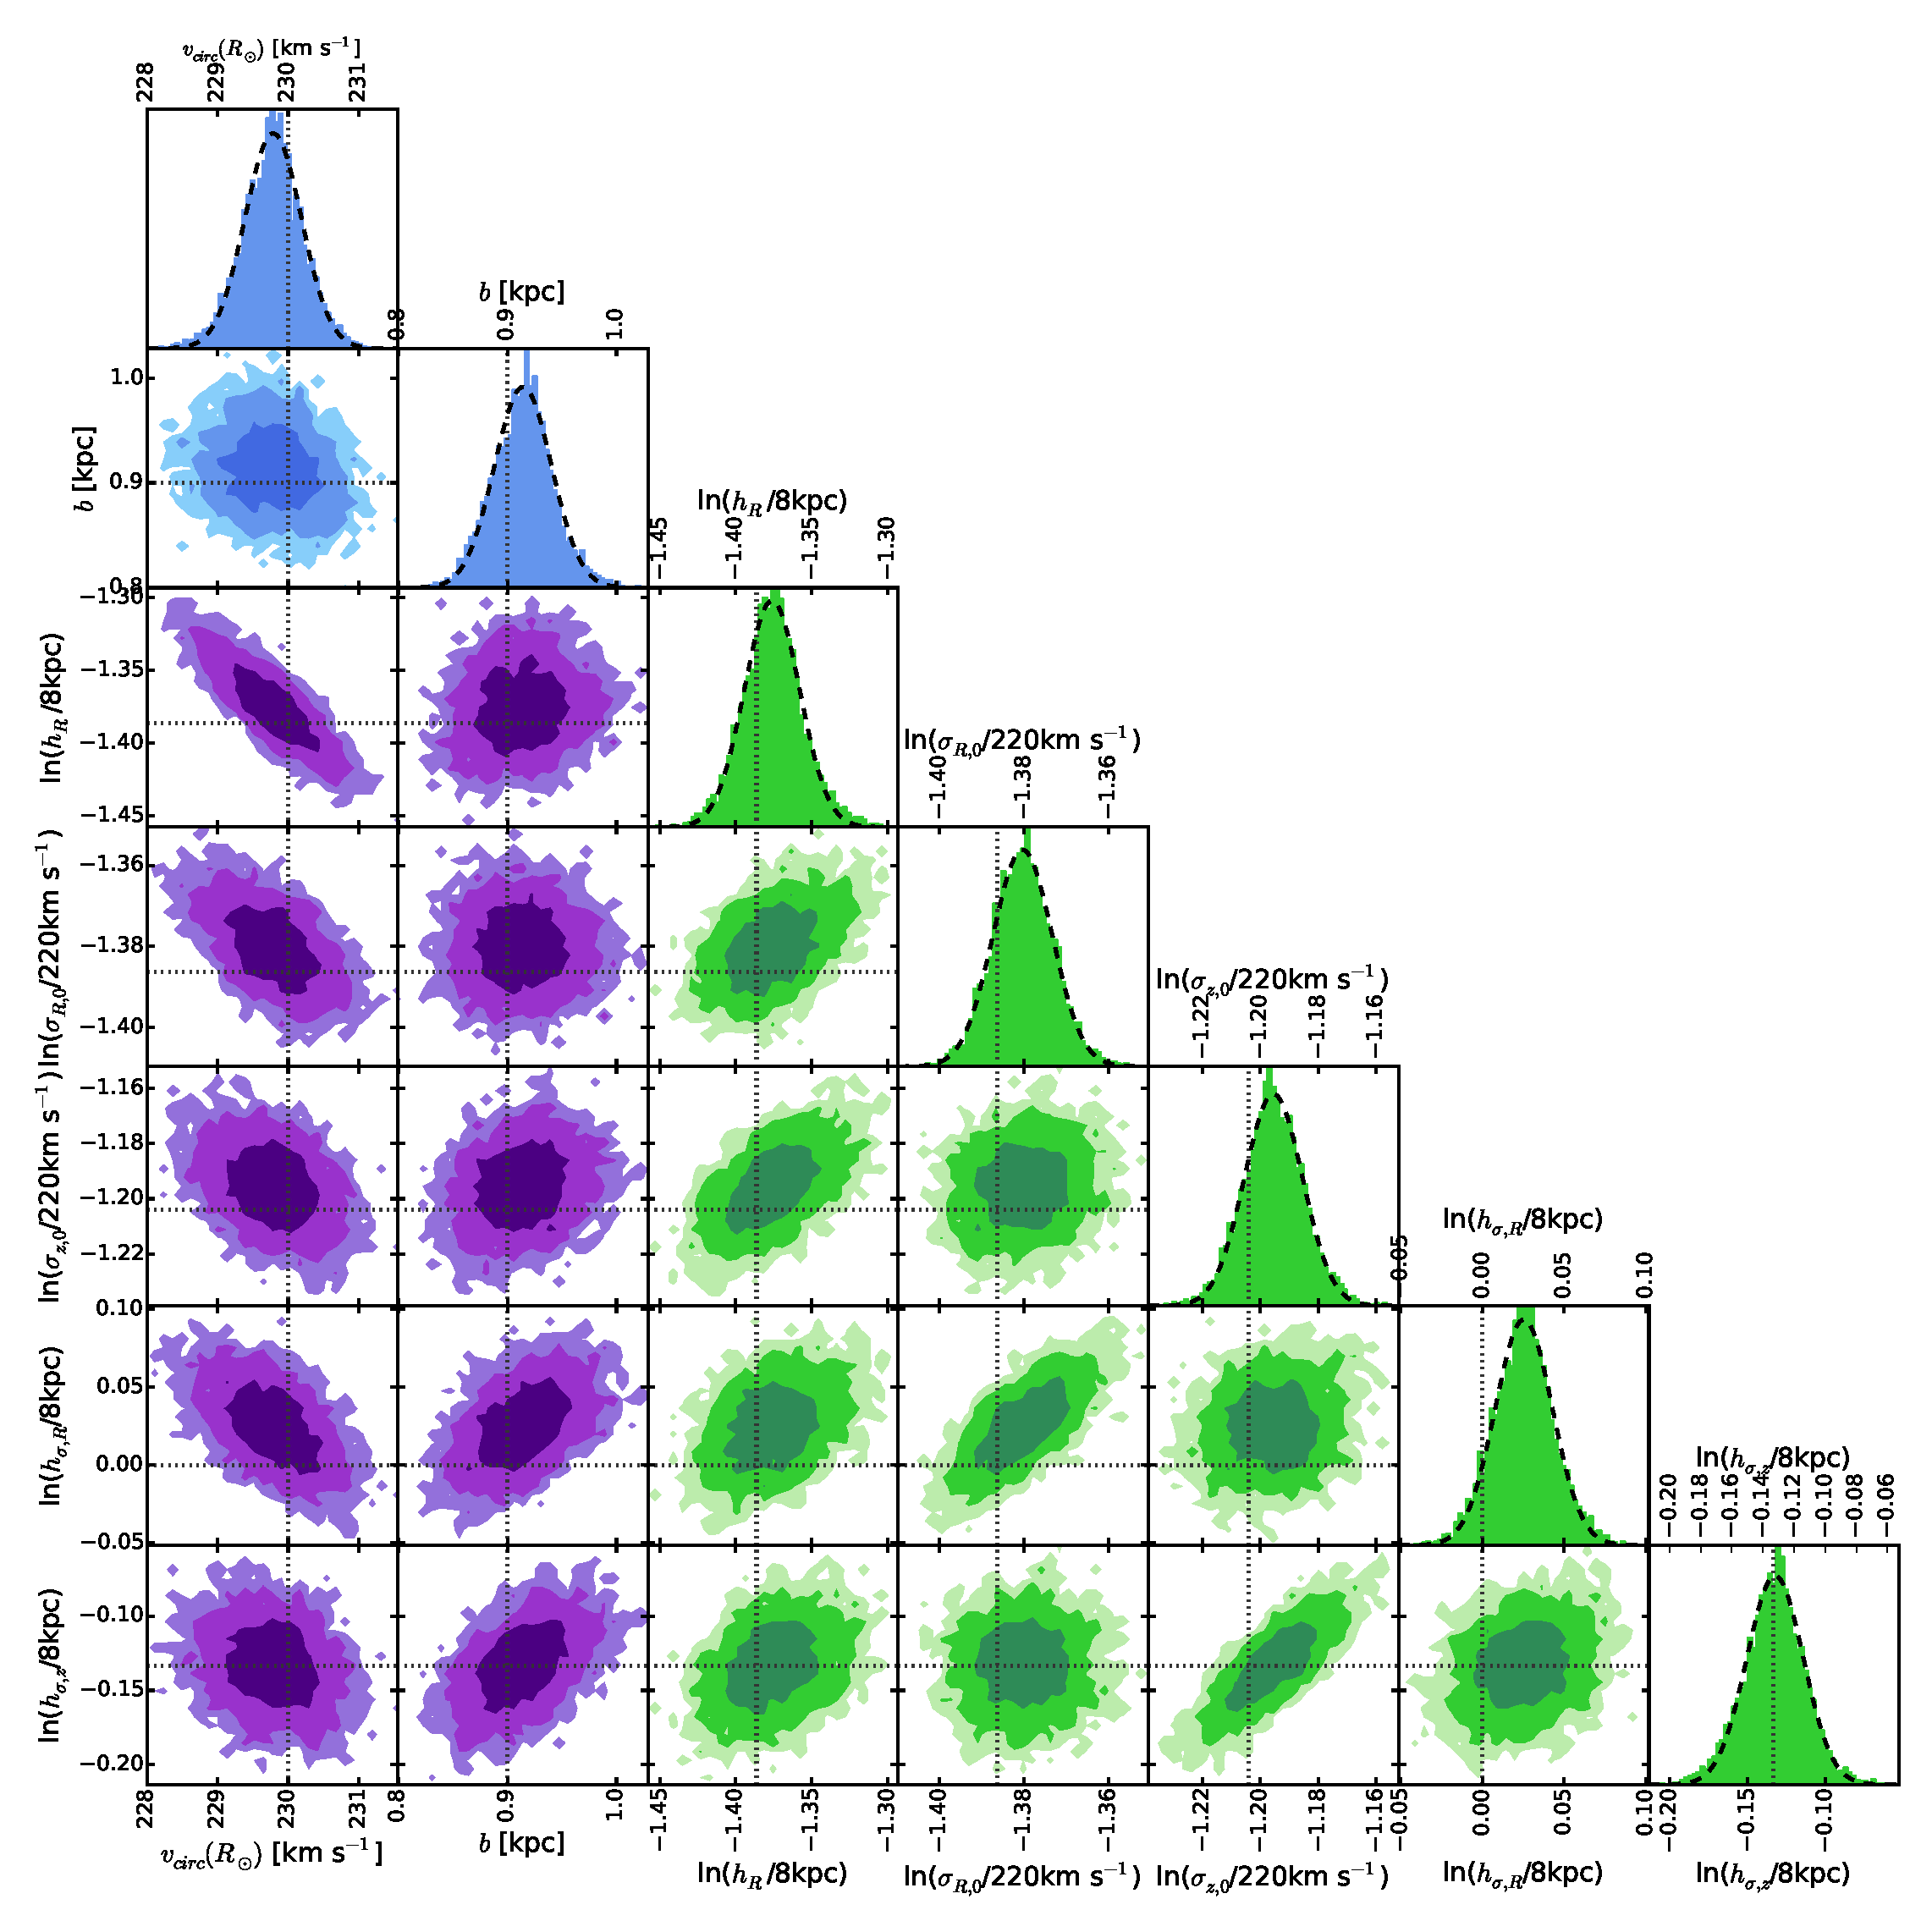
\includegraphics[width=0.7\textwidth]{figs/isoSphFlex_short_hot_2kpc_triangle_MCMC.eps}
%\plotone{figs/isoSphFlex_short_hot_2kpc_triangle_MCMC.eps}
\caption{The \pdf{} in the parameter space $\pmodel{} = \{p_\Phi,p_\text{DF}\}$ for one example mock data set created according to Test \ref{test:isoSphFlex} in Table \ref{tbl:tests}. Blue indicates the \pdf{} for the potential parameters, green the qDF parameters. The true parameters are marked by dotted lines. The dark, medium and bright contours in the 2D distributions represent 1, 2 and 3 sigma confidence regions \HW{[TO DO: HW: "likelihood vs. pdf - This is where this matters: is this a confidence on the data or on the parameters?" Don't understand, what he means...]}, respectively, and show weak or moderate covariances. This analysis was picked among five similar analyses, to have all 1 sigma contours encompass the input values \Jo{[TO DO: Jo didn't understand this sentence]}. The \pdf{} here was sampled using MCMC (with flat priors in $p_\Phi$ and  $\ln(p_\text{DF})$ to turn the likelihood in Equation \ref{eq:prob} into a full \pdf{}). Because only 10,000 MCMC samples were used to create the histograms shown, the 2D distribution has noisy contours. The dashed lines in the 1D distributions are Gaussian fits to the histogram of MCMC samples. This demonstrates very well that for such a large number of stars, the \pdf{} approaches the shape of a multi-variate Gaussian, as expected from the central limit theorem \Jo{[TO DO: Jo wrote, that he is not sure if the central limit theorem is directly relevant here]}. \Wilma{[TO DO: rename $h_{\sigma R}$ to $h_{\sigma,R}$, $\sigma_R$ to $\sigma_{R,0}$ and analogous for $z$]}}
\label{fig:isoSphFlex_triangleplot}
\end{figure*}

%====================================================================

%FIGURE: width of likelihood propto 1/sqrt(N)

\begin{figure}
\plotone{figs/sqrtNiso_Stddev_Vs_N.eps}[p]
\caption{The width of the \pdf{} for two fit parameters found from analyses of 132 mock data sets vs. the number of stars in each data set. The mock data was created in the \texttt{Iso-Pot} potential and all model parameters are given as Test \ref{test:sqrtNiso} in Table \ref{tbl:tests}. The \pdf{} (using the likelihood in Equation \ref{eq:prob} \Wilma{[TO DO: CHECK]}) was evaluated and then a Gaussian was fitted to the marginalized \pdf{} of each free fit parameter. The standard error (SE) of these best fit Gaussians is shown for the potential parameter $b$ in kpc (red dots) and for the qDF parameter $\ln(h_R/8\text{kpc})$ in dimensionless units (blue). The black lines are fits of the functional form SE$(N_\text{sample}) \propto 1/\sqrt{N_\text{sample}}$ to the data points of both shown parameters. As can be seen, for large data samples the width of the \pdf{} behaves as expected and scales with $1/\sqrt{N_\text{sample}}$ as predicted by the central limit theorem. \Wilma{[TO DO: fancybox Legend] [TO DO: write pdf instead of likelihood on y-axis]}} 
\label{fig:sqrtNiso}
\end{figure}

%====================================================================


%FIGURE: central limit theorem is satisfied

\begin{figure}[p]
\plotone{figs/isoSph_CLT_2.eps}
\caption{(Un-)bias of the parameter estimates: According to the central limit theorem the the best fit values for a large number of data sets, each containing a large number of stars, will follow the Normal distribution. To test this, we create 320 mock data sets, which come from two different stellar populations and five spherical observation volumes (see legends). All model parameters are summarized in Table \ref{tbl:tests} as Test \ref{test:isoSph_CLT}. Bias and relative standard error (SE) are derived from the marginalized \pdf{} for one potential parameter (isochrone scale length $b$ in first row) and one qDF parameter ($h_{\sigma,z}$ in second row). The second column displays a histogram of the 320 offsets. As it closely follows a Normal distribution, our modelling method is therefore well-behaved and unbiased. For the 32 analyses belonging to one model we also determine the mean offset and SE, which are overplotted in black in the first two columns (with $1/\sqrt{32}$ as error).  \HW{[TO DO: Is the scatter of the black symbols too large??? Is the reason for this numerical inaccuracies???]} \Wilma{[TO DO: Change test table accordingly, isochrone with b = 1.5 is not used anymore] [TO DO: Caption is too long. Make shorter.] [TO DO: $r_\text{max}$ instead of radius in legend] [TO DO: Leerzeichen fehlt in y-achsenbeschriftung]}}
\label{fig:isoSph_CLT}
\end{figure}

%====================================================================

\HW{[TO DO: I sometimes talk about pdf, sometimes about likelihood. We should make this consistent everywhere. I would use \pdf everywhere, but I sometimes reference the likelihood equation. How should I write it in this case?]}
\subsection{The Role of the Survey Volume Geometry} \label{sec:results_obsvolume}

To explore the role of the survey volume (see Section \ref{sec:intro}) at given sample size, we devise two suites of mock data sets: 
\\The first suite draws mock data from the same \pmodel{}, {\it two different potentials} (\texttt{Iso-Pot} and \texttt{MW13-Pot}, see Test \ref{test:wedFlexVol} in Table \ref{tbl:tests}), and volume wedges (see Section \ref{sec:selectionfunction}) at {\it different positions within the Galaxy}, illustrated in the right upper panel of Figure \ref{fig:wedFlexVol_bias_vs_SE}. To isolate the role of the survey volume geometry, the mock data sets are equally large (20,000) in all cases, and are drawn from identical total survey volumes ($4.5~\text{kpc}^3$, achieved by adjusting the angular width of the wedges). The results are shown in Figure \ref{fig:wedFlexVol_bias_vs_SE}.
\\The second suite of mock data sets was already introduced in Section \ref{sec:largedata} (see also Test \ref{test:isoSph_CLT}), where mock data sets were drawn from five spherical volumes around the sun with different maximum radius, for {\it two different stellar populations}. The results of this second suite are shown in Figure \ref{fig:isoSph_CLT} and demonstrate the effect of the {\it size of the survey volume}.
\\Figures \ref{fig:isoSph_CLT} and \ref{fig:wedFlexVol_bias_vs_SE} illustrate the ability of \RM{} to constrain model parameters, with the standard error of the \pdf{} as measure of the precision on the $x$-axis. Figure \ref{fig:isoSph_CLT} demonstrates that, given a choice of qDF, a larger volume always results in tighter constraints. There is no obvious trend that a hotter or cooler \MAP{} will always give better results \HW{[TO DO: Comment from HW: The question of whether a hotter or a colder population gives tighter constraints is an important question, but it seems buries here in a section that is dedicated to another matter, namely the question of volume ... It's OK to leave it here, but somewhere we need to say clearly: whether the population is hot or cold does not make a big and generic difference...]}; it depends on the survey volume and the model parameter in question. In Figure \ref{fig:wedFlexVol_bias_vs_SE} the wedges all have the same volume and all give results of similar precision. Minor differences, e.g. with the \texttt{Iso-Pot} potential being less constrained in the wedge with large vertical, but small radial extent, are a special property of the considered potential and parameters, and not a global property of the corresponding survey volume. In the case of an axisymmetric model galaxy, the extent in $\phi$ direction is not expected to matter. Overall radial extent and vertical extent seem therefore to be equally important to constrain the potential. In addition Figure \ref{fig:wedFlexVol_bias_vs_SE} implies that for these cases volumes offsets in the radial or vertical direction have at most a modest impact - even in case of the very large sample size at hand.
\\While it appears that the argument for significant radial and vertical extent is generic, we have not done a full exploration of all combinations of \pmodel{} and volumina.

%====================================================================

%FIGURE: Does shape and position of obs. volume matter?


\begin{figure*}[p]
\plotone{figs/wedFlexVol_bias_vs_SE.eps}
\caption{Bias vs. standard error in recovering the potential parameters for mock data stars drawn from four different test observation volumes within the Galaxy (illustrated in the upper right panel) and two different potentials (\texttt{Iso-Pot} and \texttt{MW13-Pot} from Table \ref{tbl:referencepotentials}). Standard error and offset were determined as in Figure \ref{fig:isoSph_CLT}. Per volume and potential we analyse four different mock data realisations; all model parameters are givenas Test \ref{test:wedFlexVol} in Table \ref{tbl:tests}. The colour-coding represents the different wedge-shaped observation volumes. The angular extent of each wedge-shaped observation volume was adapted such that all have the volume of $4.5 \text{ kpc}^3$, even though their extent in $(R,z)$ is different.  Overall there is no clear trend, that an observation volume around the sun, above the disk or at smaller Galactocentric radii should give remarkably better constraints on the potential than the other volumes. [TO DO: Write in Plot "... that all wedges have the same volume".]}
\label{fig:wedFlexVol_bias_vs_SE}
\end{figure*}


%====================================================================

\subsection{The Significance of Incorrect assumptions on the (In-)Completeness of the Data Set} \label{sec:results_incompR}

The selection function of a survey could be described by a spatial survey volume and a completeness function, which determines the fraction of stars observed at a given location within the Galaxy with a given brightness, metallicity etc (see \S\ref{sec:selectionfunction}). The completeness function depends on the characteristics and mode of the survey, can be very complex and is therefore sometimes not perfectly known. We investigate how much an imperfect knowledge of the selection function can affect the recovery of the potential. We model this by creating mock data with varying incompleteness, while assuming constant completeness in the analysis. The mock data comes from a sphere around the sun and an incompleteness function that drops linearly with distance $r$ from the sun (see Test \ref{test:isoSphFlexIncomp}, Example 1, in Table \ref{tbl:tests} and Figure \ref{fig:isoSphFlexIncompR_mockdata}).
\\This could be understood as a model for the important effect of stars being less likely to be observed the further away they are. We demonstrate that the potential recovery with \RM{} is very robust against somewhat wrong assumptions about the (in-)completeness of the data (see Figure \ref{fig:isoSphFlexIncompR_violins}). A lot of information about the potential comes from the rotation curve measurements in the plane, which is not affected by applying an incompleteness function. In Appendix \S\ref{sec:incompZ} we also show that the robustness is somewhat less striking but still given for small misjudgments of the incompleteness in vertical direction, parallel to the disk plane (Figures \ref{fig:isoSphFlexIncompZ_mockdata} and \ref{fig:isoSphFlexIncompZ_violins}). This could model the effect of wrong corrections for dust obscuration in the plane. We also investigate in Appendix \S\ref{sec:incompZ} if indeed most of the information is stored in the rotation curve. For this we use the same mock data sets as analysed in Figures \ref{fig:isoSphFlexIncompR_violins} and \ref{fig:isoSphFlexIncompZ_violins}, but this time we’re not including the tangential velocities in the modelling, rather marginalizing the likelihood over $v_T$. In this case the potential is much less tightly constrained, even for 20,000 stars. For only small deviations of true and assumed completeness ($\lesssim 10\%$) we can however still incorporate the true potential in our fitting result (see Figure \ref{fig:isoSphFlexIncomp_marginal_violins}). 



%FIGURE: isoSphFlexIncompR in mock data space

\begin{figure}
\includegraphics[width=\columnwidth]{figs/isoSphFlexIncompR_mockdata.eps}
\caption{Selection function and mock data distribution for investigating radial incompleteness of the data. All model parameters are summarized as Test \ref{test:isoSphFlexIncomp}, Example 1, in Table \ref{tbl:tests}. The survey volume is a sphere around the sun and the percentage of observed stars is decreasing linearly with radius from the sun, as demonstrated in the left panel. How fast this detection/incompleteness rate drops is quantified by the factor $\epsilon_r$. Histograms for four data sets, drawn from two \MAPs{} (\texttt{hot} in red and \texttt{cool} in blue, see Table \ref{tbl:referenceMAPs}) and with two different $\epsilon_r$, 0 and 0.7, are shown in the right panel for illustration purposes. [TO DO: Potential and/or population names in typewriter font]} 
\label{fig:isoSphFlexIncompR_mockdata}
\end{figure}

%FIGURE: isoSphFlexIncompR

\begin{figure*}
\centering
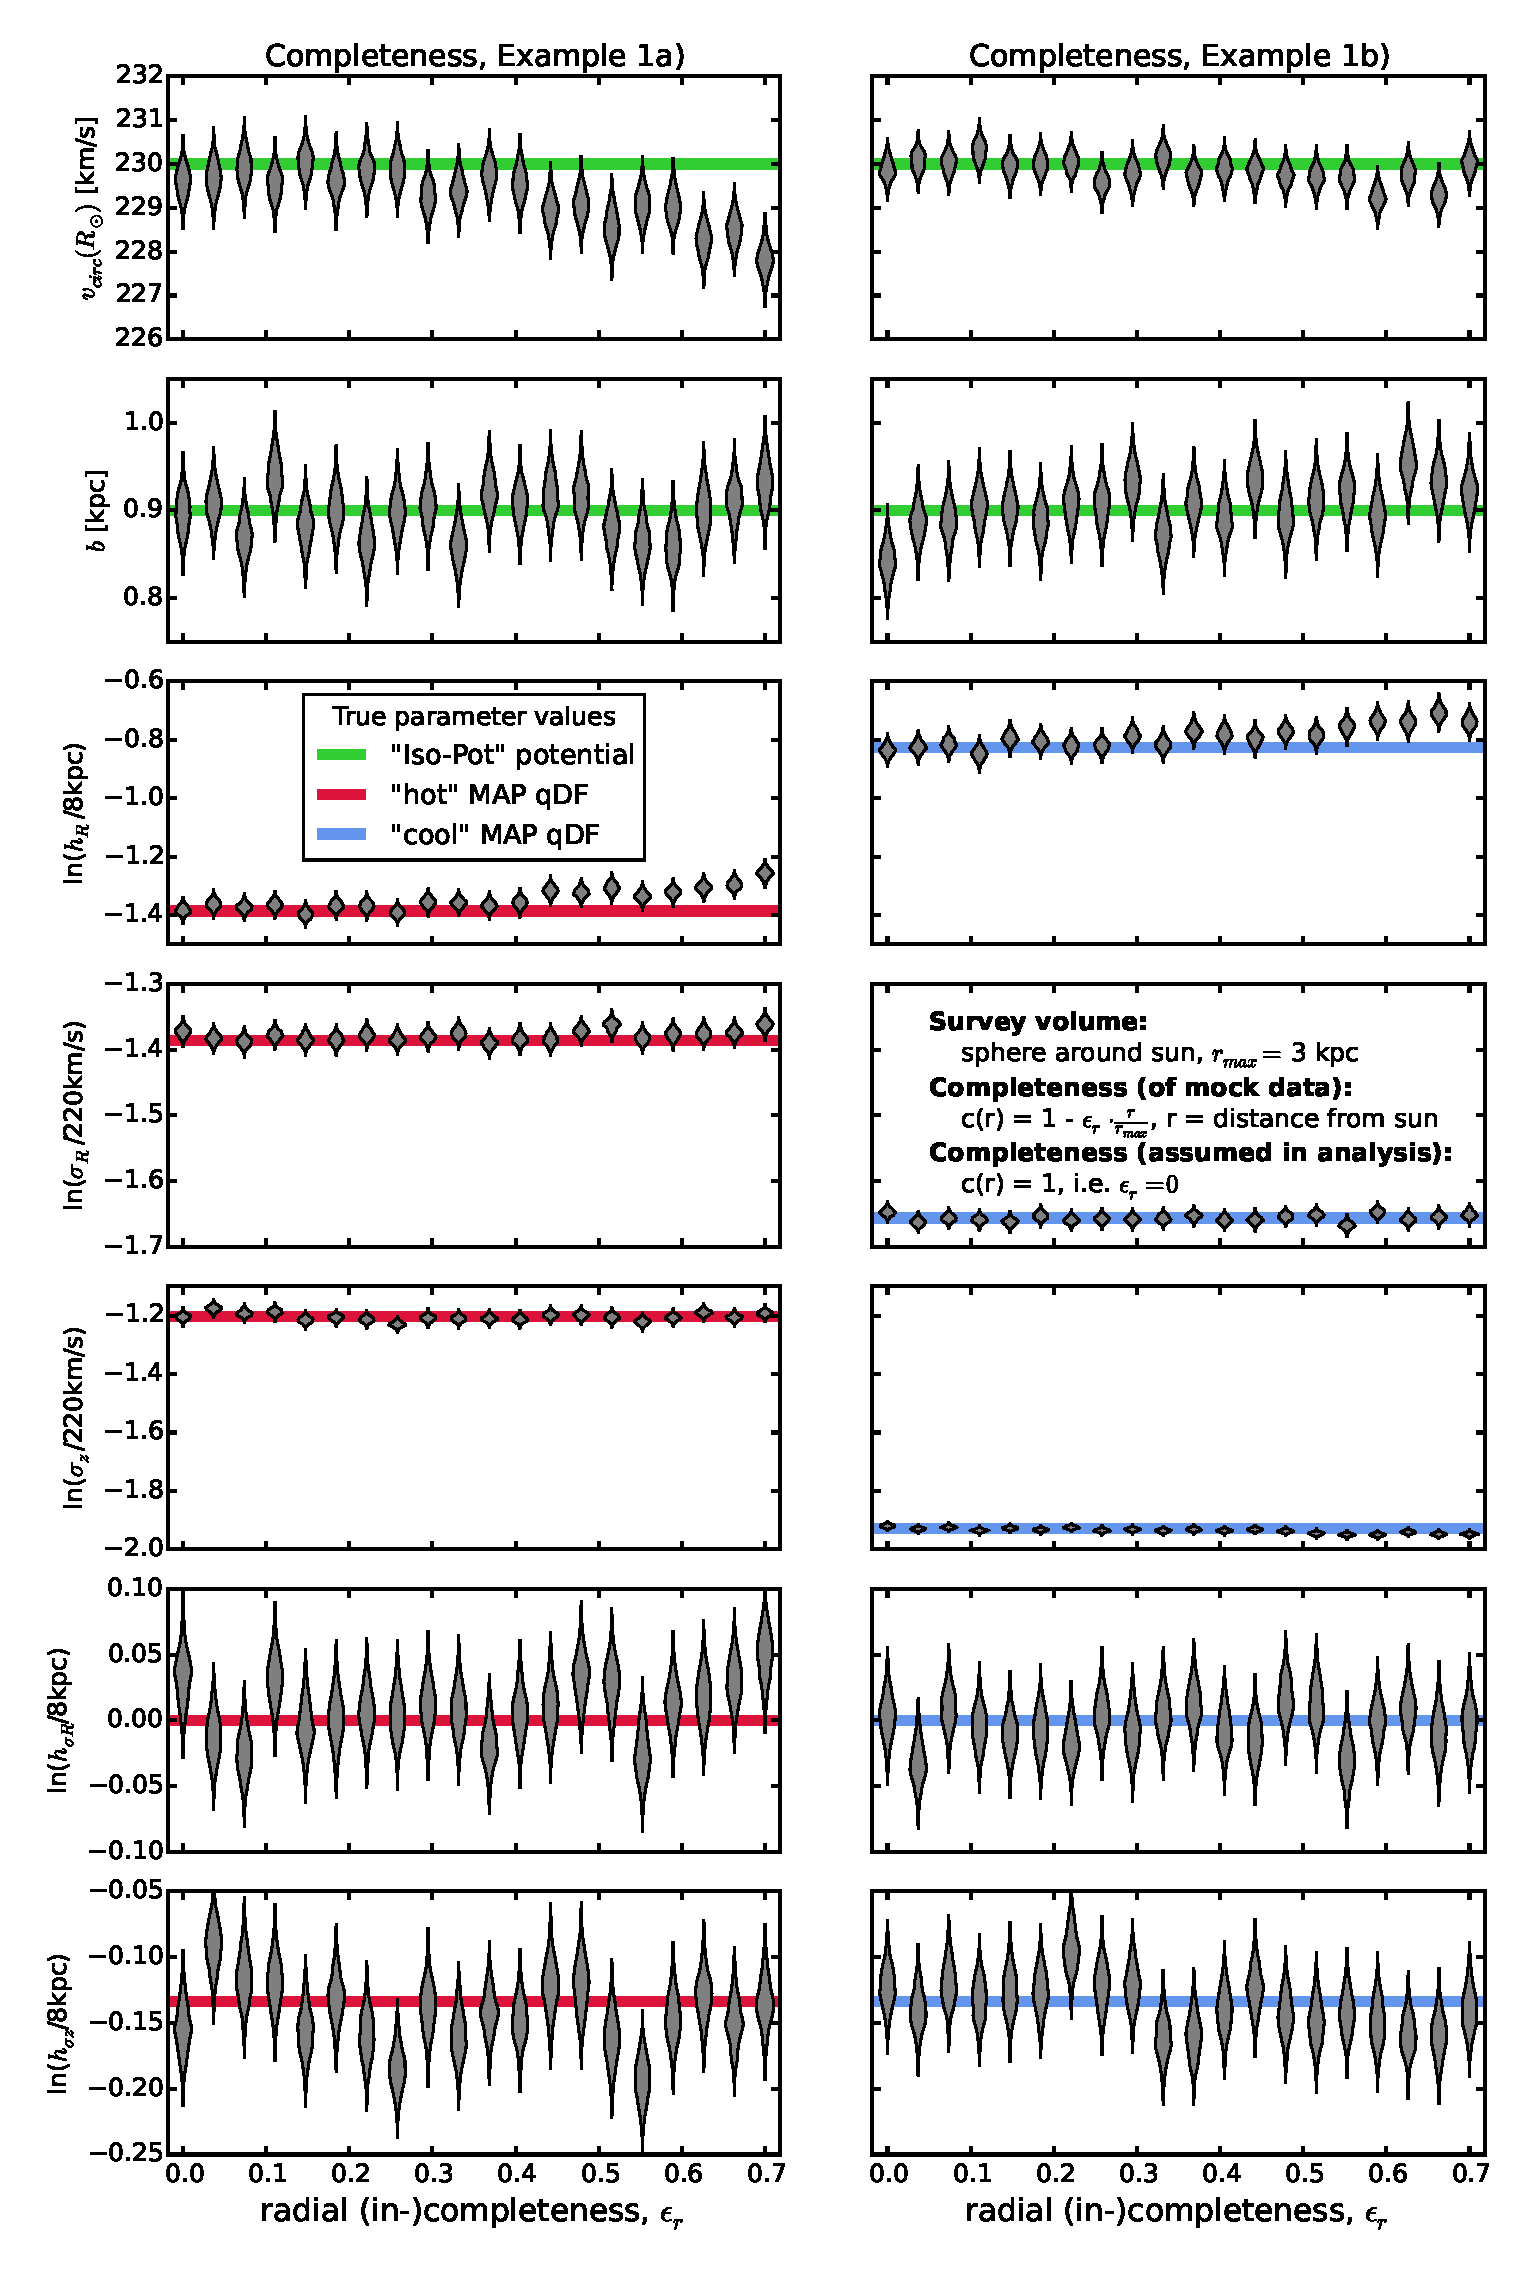
\includegraphics[width=0.8\textwidth]{figs/isoSphFlexIncompR_violins.eps}
\caption{(Caption on next page.)}
\end{figure*}


\addtocounter{figure}{-1}
\begin{figure*} [t!]
\caption{Influence of wrong assumptions about the radial incompleteness of the data on the parameter recovery with \RM{}. Each mock data set was created having different incompleteness parameters $\epsilon_r$ (shown on the $x$-axis and illustrated in Figure \ref{fig:isoSphFlexIncompR_mockdata}) and the model parameters are given as Test \ref{test:isoSphFlexIncomp}, Example 1, in Table \ref{tbl:tests}. The analysis however didn't know about the incompleteness and assumed that all data sets had constant completeness within the survey volume ($\epsilon_r = 0$). The marginalized likelihoods from the fits are shown as violins. The green lines mark the true potential parameters (\texttt{Iso-Pot}) and the red and blue lines the true qDF parameters (\texttt{hot} \MAP in red and \texttt{cool} \MAP in blue), which we tried to recover. The \RM{} method seems to be very robust against small to intermediate deviations between the true and the assumed data incompleteness. [TO DO: rename $h_{\sigma R}$ to $h_{\sigma,R}$, $\sigma_R$ to $\sigma_{R,0}$ and analogous for $z$] [TO DO: Potential and/or population names in typewriter font]} 
\label{fig:isoSphFlexIncompR_violins}
\end{figure*}


\subsection{Dealing with Measurement Errors and their Effect on the Parameter Recovery} \label{sec:results_errors}

\paragraph{Convergence of the error integral.} In \S \ref{sec:likelihood} we introduced how we convolve the model probability with the measurement errors. In the absence of distance errors the accuracy of the parameter recovery is limited by an insufficient MC sampling of the convolution integral in Equation (\ref{eq:errorconv}). Test \ref{test:isoSphFlexErrConv_MC_vs_error} in Table \ref{tbl:tests} and Figure \ref{fig:isoSphFlexErrConv_MC_vs_error} investigate how many MC samples are needed, given the size of the velocity error, for the integral to be accurate within certain limits:
\\For each $\delta \mu \in [2,3,4,5] \text{mas yr}^{-1}$ we set up four mock data sets and evaluated the likelihood for different $N_\text{error}$. We used $N_\text{conv} :=$ 800 and 1200 MC samples to calculate the numerically converged likelihood for proper motion errors $\delta \mu \leq 3 \text{mas yr}^{-1}$ and $\delta \mu > 3 \text{mas yr}^{-1}$, respectively (see left panels in Figure \ref{fig:isoSphFlexErrConv_bias_vs_SE}). We determined the mean bias 
\begin{equation*}
\text{BIAS}(N_\text{error},\delta \mu) \equiv \frac{1}{4} \sum_{j=1}^4 \left[ \langle p_i \rangle (N_\text{error},\delta \mu)\right]_j - \left[ \langle p_i \rangle (N_\text{conv},\delta \mu)\right]_j,
\end{equation*}
where $\left[ \langle p_i \rangle (N_\text{error},\delta \mu)\right]_j$ is the best estimate for the $i$-th model parameter $p_i \in \pmodel$ from the analysis of the $j$-th mock data realisation with $\delta \mu$ using $N_\text{error}$ MC samples. From this we then generated the curves $N_{\text{error},i} (\delta v_\text{max},\text{BIAS})$ in Figure \ref{fig:isoSphFlexErrConv_MC_vs_error} by linear interplolation, that show how many MC samples are needed for parameter $p_i$ given a velocity error and a systematic bias in units of the standard error (SE) of the estimate. The proper motion error $\delta \mu$ translates to a velocity error according to 
\begin{equation}
\delta v_\text{max} [\text{km s}^{-1}] \equiv 4.74047 \cdot r_\text{max}[\text{kpc}] \cdot \delta \mu [\text{mas yr}^{-1}], \label{eq:vmax}
\end{equation}
where $r_\text{max}$ is the maximum distance of stars. We find in Figure \ref{fig:isoSphFlexErrConv_MC_vs_error} the relation
\begin{equation*}
N_{\text{error},i} (\delta v_\text{max},\text{BIAS}) \propto \left( \delta v_\text{max} \right)^2.
\end{equation*}
Figure \ref{fig:isoSphFlexErrConv_MC_vs_error} also demonstrates that different model parameters do not have the same sensitivity to the numerical inaccuracies introduced by insufficient sampling. [TO DO: we haven't tested yet, if this plot depends on hotness of population and / or number of stars. But if it takes forever to actually do the calculations, I guess, we just leave it like this.]

\paragraph{Testing the error convolved likelihood approximation.} In absence of distance (modulus) errors our approximation for the likelihood, which is the model probability convolved with the measurement errors in Equation (\ref{eq:errorconv}), is equal to the true likelihood. In case there \emph{are} distance modulus errors, this likelihood links the range of possible velocities (specified by the measurement errors in line-of-sight velocity, proper motion and distance modulus) to a fixed but slightly wrong position, as we ignore the distance error in the position. As the link between position and velocity provides the information about the potential, this will lead to systematic biases in the parameter recovery the larger the distance error becomes. In Test \ref{test:isoSphFlexErrConv_bias_vs_SE} in Table \ref{tbl:tests} and Figure \ref{fig:isoSphFlexErrConv_bias_vs_SE} we investigate the capabilities of Equation (\ref{eq:errorconv}) with and without distance modulus errors.
\\The left column of panels in Figure \ref{fig:isoSphFlexErrConv_bias_vs_SE} shows how well the approximation works in the absence of distance errors. There seemed to be no biases in the parameter recovery, independent of the size of the proper motion error. (We note that there could be a tiny bias $\ll 1$ SE in the $\ln(\sigma_{z,0} / 200\text{ km s}^{-1})$ qDF parameter, most likely due to insufficient numerical accuarcy, but all the other model parameters, also those not shown in the figure, are very well behaved.) Overall the standard errors on the recovered parameters are quite small (a few percent at most for 10,000 stars), which demonstrates that, if we perfectly knew the measurement errors, we still could get very precise constraints on the potential. The constraints also get tighter the smaller the proper motion error becomes. We found that for $\delta \mu = 1 \text{ mas yr}^{-1}$ the precision of the recovered parameters reduce by $\sim$ half compared to $\delta \mu = 5 \text{ mas yr}^{-1}$.
\\The right column of panels in Figure \ref{fig:isoSphFlexErrConv_bias_vs_SE} demonstrates the failure of our adopted likelihood approximation in the case of large distance modulus errors. The larger the $\delta(m-M)$, the wronger the recovered parameters become: The systematic biases can get many SEs large. We find however that in case of $\delta(m-M) \leq 0.2 \text{ mag}$ (if also $\delta \mu \leq 2 \text{ mas yr}^{-1}$ and a maximum distance of $r_\text{max} = 3 \text{ kpc}$, see Test \ref{test:isoSphFlexErrConv_bias_vs_SE} in Table \ref{tbl:tests}) the parameters can still be recovered within 2 SEs. For most model parameters (except $\ln(\sigma_{z,0} / 200\text{ km s}^{-1})$, as shown in the figure, and $\ln(h_R/ 8\text{ kpc})$) even $\delta(m-M) \leq 0.3 \text{ mag}$ still gives biases smaller than 2 SEs. This corresponds to a relative distance error of $\sim10\%$. This encourages us that for smaller distance modulus errors we really could use our likelihood approximation in Equation (\ref{eq:errorconv}), which is computationally cheaper than a proper treatment, also on real data sets.



\paragraph{Underestimation of the proper motion error.} We found that in case we perfectly knew the measurement errors (and the distance error is negligible), the convolution of the model probability with the measurement errors gives precise and accurate constraints on the model parameters - even if the error itself is quite large. Now we investigate what would happen if the quoted measurement errors, e.g. the proper motion errors, were actually smaller than the true errors. Figure \ref{fig:isoSphFlexErrSyst} shows the case for two different stellar populations and an error underestimation of 10\% and 50\%. 
\\Overall the parameter recovery gets worse the larger the proper motion error and the stronger the underestimation. The relation between the bias due to error misjudgment and the size of the proper motion error seems to be linear.
\\For the recovery of the isochrone potential scale length $b$ the hotness of the population does not matter (see lower left panel in Figure \ref{fig:isoSphFlexErrSyst}). The circular velocity $v_\text{circ}(R_\odot)$ is, as always, better measured by cooler than by hotter populations (see upper left panel in Figure \ref{fig:isoSphFlexErrSyst}). 
\\We find that the recovery of the qDF parameters on the other hand is more strongly affected by the misjudgment of the velocity error for \emph{cooler} stellar popluations. The measured velocity dispersion is the convolution of the intrinsic dispersion with the measurement errors. If the proper motion error is underestimated, the deconvolved velocity dispersion is larger than the intrinsic velocity dispersion and the relative difference is bigger for a cooler population (see upper right panel for $\sigma_{z,0}$ in Figure \ref{fig:isoSphFlexErrSyst}). The intrinsic velocity dispersion is also cooler at larger radii than at smaller radii, therefore the deconvolved dispersion is overestimated more strongly at large $R$ and the velocity dispersion scale length will be overestimated as well (see lower left panel for $h_{\sigma,z}$ in Figure \ref{fig:isoSphFlexErrSyst}). We get analogous results for the qDF parameters $\sigma_{R,0}$ and $h_{\sigma,R}$. The recovery of the tracer density scale length $h_R$ is not affected by the misjudgment of velocity errors. 
\\The most important and encouraging result from Figure \ref{fig:isoSphFlexErrSyst} is, that for an underestimation of $10\%$ the bias is still $\lesssim 2$ sigma [TO DO: can I say sigma???] - even for proper motion errors of almost $3$ mas/yr.

%=============================================================

\begin{figure}
\plotone{figs/isoSphFlexErrConv_MC_vs_error.eps}
\caption{Number of Monte Carlo (MC) samples $N_\text{error}$ needed for the numerical error convolution in Equation (\ref{eq:errorconv}), given the maximum velocity error $\delta v_\text{max}$ in the sample to reach a given accuracy.  An insufficient sampling of the convolution integral leads to systematic biases in the reconstruction of the true model parameters. The size of the bias is color coded as indicated in the legend and is given in units of the standard error (SE).  The model parameters, marked by different symbols, have different sensitivities to the numerical inaccuracy of the error convolution, therefore the range in $N_\text{error}$ for the same given bias. Here we assume that the distance error is zero and the proper motion error $\delta \mu$ translates to a velocity error according to Equation (\ref{eq:vmax}) and $\delta v_\text{los} \ll \delta v_\text{max}$. All model parameters are listed in Table \ref{tbl:tests} as Test \ref{test:isoSphFlexErrConv_MC_vs_error}. The number of MC samples needed increases with the velocity error as $N_\text{error} \propto \left( \delta v_\text{max} \right)^2$, as can be seen especially well in the inset figure for the potential parameter $v_\text{circ}(R_\odot)$. All lines are fits of this functional form to each four points derived for a given model parameter (symbol) and bias (color). The large scatter in the points comes from low number statistics and errors introduced by linear interpolation of the bias vs. $N_\text{error}$ relation found from the analyses. [TO DO: rename $h_{\sigma R}$ to $h_{\sigma,R}$, $\sigma_R$ to $\sigma_{R,0}$ and analogous for $z$] [TO DO: some of the 25 MC sample analyses have to be re-done. (Currently running on cluster.)]}
\label{fig:isoSphFlexErrConv_MC_vs_error}
\end{figure}


%=============================================================

\begin{figure}
\plotone{figs/isoSphFlexErrConv_bias_vs_SE.eps}
\caption{(Caption on next page.)}
\end{figure}

\addtocounter{figure}{-1}
\begin{figure} [t!]
\caption{Parameter recovery using the approximation for the measurement error convolved likelihood in Equation (\ref{eq:errorconv}). All model parameters used to create the mock data sets analyzed for this figure are given as Test \ref{test:isoSphFlexErrConv_bias_vs_SE} in Table \ref{tbl:tests}. The mock data sets in the left panels have only errors in line-of-sight velocity and proper motions, while the data sets in the right panels also have distance modulus errors, as indicated in the legends in the first row. The size of the error is color coded. The other panels plot the offset of the recovered model parameter to the true parameter vs. the relative standard error for two of the seven model parameters, the potential parameter $v_\text{circ}(R_\odot)$ and qDF parameter $\sigma_{z,0}$. For data sets with proper motion error errors $\delta(m-M) \leq 3 \text{mas yr}^{-1}$ Equation (\ref{eq:errorconv}) was evaluated with $N_\text{error}=800$, for $\delta(m-M) > 3 \text{mas yr}^{-1}$ we used $N_\text{error}=1200$. In the absence of distance errors Equation (\ref{eq:errorconv}) gives unbiased results, for $\delta(m-M) \geq 3 \text{mas yr}^{-1}$ (which corresponds in this test to $\delta v_\text{max} \lesssim 43$, see Equation (\ref{eq:vmax})) however biases of several sigma [TO DO: can I say sigma???] are introduced as Equation (\ref{eq:errorconv}) in only an approximation for the true likelihood in this case. [TO DO: rename  $\sigma_z$ to $\sigma_{z,0}$]}
\label{fig:isoSphFlexErrConv_bias_vs_SE}
\end{figure}




%=============================================================

\begin{figure}
\plotone{figs/isoSphFlexErrSyst_offset_vs_error.eps}
\caption{Effect of an systematic underestimation of proper motion errors in the recovery of the model parameters. The true model parameters used to create the mock data are summarized as Test \ref{test:isoSphFlexErrSyst} in Table \ref{tbl:tests}, four of them are given on the $y$-axes and the true values are indicated as black dashed lines. The velocities of the mock data were perturbed according to Gaussian errors in the $\alpha$ and $\delta$ proper motions as indicated on the $x$-axis.   The circles and triangles are the best fit parameters of several mock data set assuming the proper motion error, with which the model probability was convolved, was underestimated in the analysis by 10\% or 50\%, respectively. The error bars correspond to 1 sigma [TO DO: Can I say sigma????] confidence. The lines connect the mean of each two data realisations and are just guides to the eyes. [TO DO: rename $h_{\sigma z}$ to $h_{\sigma,z}$, $\sigma_z$ to $\sigma_{z,0}$] [TO DO: Potential and/or population names in typewriter font]}
\label{fig:isoSphFlexErrSyst}
\end{figure}

%=============================================================
%\subsection{The Impact of Deviations of the Data from the Idealized qDF} \label{sec:results_mixedDFs}

%Motivation of the test and what we're doing
Our modelling approach assumes that each \MAP{} follows a quasi-isothermal distribution function, qDF. In this Section we explore what happens if this idealization does not hold. We investigate this issue by creating mock data sets (Figure \ref{fig:isoSphFlexMix_mockdata_residuals}) that are drawn from two distinct qDFs of different temperature, and analyze the composite mock data set by fitting a single qDF to it. These results are illustrated in Figures \ref{fig:isoSphFlexMixCont} and \ref{fig:isoSphFlexMixDiff}. Following the observational evidence, \MAPs{} with cooler qDFs also have longer tracer scale lengths. In the first set of test, we choose qDFs of widely different temperatures and vary their relative fraction (dubbed \emph{Examples 1a/b} in Figure \ref{fig:isoSphFlexMixCont} and Test \ref{test:isoSphFlexMix} in Table \ref{tbl:tests}); in the second set of tests (\emph{Examples 2a/b} in Figure \ref{fig:isoSphFlexMixDiff} and Test \ref{test:isoSphFlexMix}in Table \ref{tbl:tests}), we always mix mock data points from two different qDFs in equal proportion, but vary by how much the qDF's temperatures differ. 
\\The first set of tests mimics a DF that has wider wings or a sharper core in velocity space than a qDF (Figure \ref{fig:isoSphFlexMix_mockdata_residuals}). The second test could be understood as mixing neighbouring \MAPs{} due to large bin sizes or abundance measurement errors.

%What we see in the plot
It is worth considering the impact of the DF deviations on the recovery of the potential and of the qDF parameters separately. We find from Example 1 that the potential parameters can be better and more robustly recovered, if a mock-data \MAP{} is polluted by a modest fraction ($\lesssim 30\%$) of stars drawn from a much cooler qDF with a longer scale length, as opposed to the same pollution of stars drawn from a hotter qDF with a shorter scale length. 
\\When considering the case of a 50/50 mix of contributions from different qDFs in Example 2, there is a systematic, but only small, error in recovering the potential parameters, monotonically increasing with the qDF parameter difference; in particular for fractional differences in the qDF parameters of $\lesssim 20\%$ the systematics are insignificant even for samples sizes of 20,000, as used in the mock data. 
\\Overall, mock data drawn from a cooler DF always seem to give tighter constraints on the circular velocity at the Sun \Wilma{[TO DO: Make sure that Sun is written everywhere with a capital S.]}, because the rotation curve can be constrained easier if more stars are on near-circular orbits. But we found the recovered $v_\text{circ}(R_\odot)$ not always to be unbiased at the implied precision.
\\The recovery of the effective qDF parameters, in light of non-qDF mock data is quite intuitive: the effective qDF temperature lies between the two temperatures from which the mixed DF of the mock data was drawn; in all cases the scale length of the velocity dispersion fall-off, $h_{\sigma,R}$ and $h_{\sigma,z}$, is shorter, because the stars drawn form the hotter qDF dominate at small radii, while stars from the cooler qDF (with its longer tracer scale length) dominate at large radii. The recovered tracer scale lengths, $h_R$ vary smoothly between the input values of the two qDFs that entered the mix of mock data, with again the impact of contamination by a hotter qDF (with its shorter scale length in this case) being more important. Overall, we find that the potential inference is quite robust to modest deviations of the data from the assumed DF.



%====================================================================

%FIGURE: isoSphFlexMix_mockdata_residuals

\begin{figure*}
\plotone{figs/isoSphFlexMix_mockdata_residuals.eps}
\caption{Distribution of mock data, created by mixing stars drawn from two different qDFs (solid lines), and the distribution predicted by the best fit of a single qDF and potential to the data (dashed lines). The model parameters to create the mock data (solid lines) are given in Table \ref{tbl:tests} as Test \ref{test:isoSphFlexMix}, and the qDF parameters referenced in the figure's legend are given in Table \ref{tbl:referenceMAPs}. The corresponding single qDF best-fit curves (dashed lines) were created by drawing mock data from the best fit parameters found in Figures \ref{fig:isoSphFlexMixCont} and \ref{fig:isoSphFlexMixDiff}. \emph{Example 1:} Distribution of mock data drawn from a superposition of two very different (but fixed) qDFs at varying mixing rates. \emph{Example 2:} Mock data distribution of two \MAPs{} that were mixed at a fixed rate of 50\%/50\%, but the difference of the qDF parameters of one \MAP{} was varied with respect to the qDF parameters of the other \MAP{} by $X\%$ (see Table \ref{tbl:referenceMAPs}). The data sets are color coded in the same way as the corresponding analyses in Figures  \ref{fig:isoSphFlexMixCont} and \ref{fig:isoSphFlexMixDiff}. This figure demonstrates how mixing two qDFs can be used as a test case for changing the shape of the DF to not follow a pure qDF anymore, e.g. by adding wings or slightly changing the radial density profile. When comparing the mock data and best fit distribution, we see that especially for the most extreme deviations it becomes obvious that a single qDF is a bad assumption for the stars' \emph{true} DF. \Wilma{[TO DO: Potential and/or population names in typewriter font] [TO DO: include $X$ somehow in figure to explain it better. Jo didn't understand what I meant by it in this caption.] [TO DO: These are really many panels. Try to remove some.]}}
\label{fig:isoSphFlexMix_mockdata_residuals}
\end{figure*}


%FIGURE: isoSphFlexMixCont

\begin{figure*}
\centering
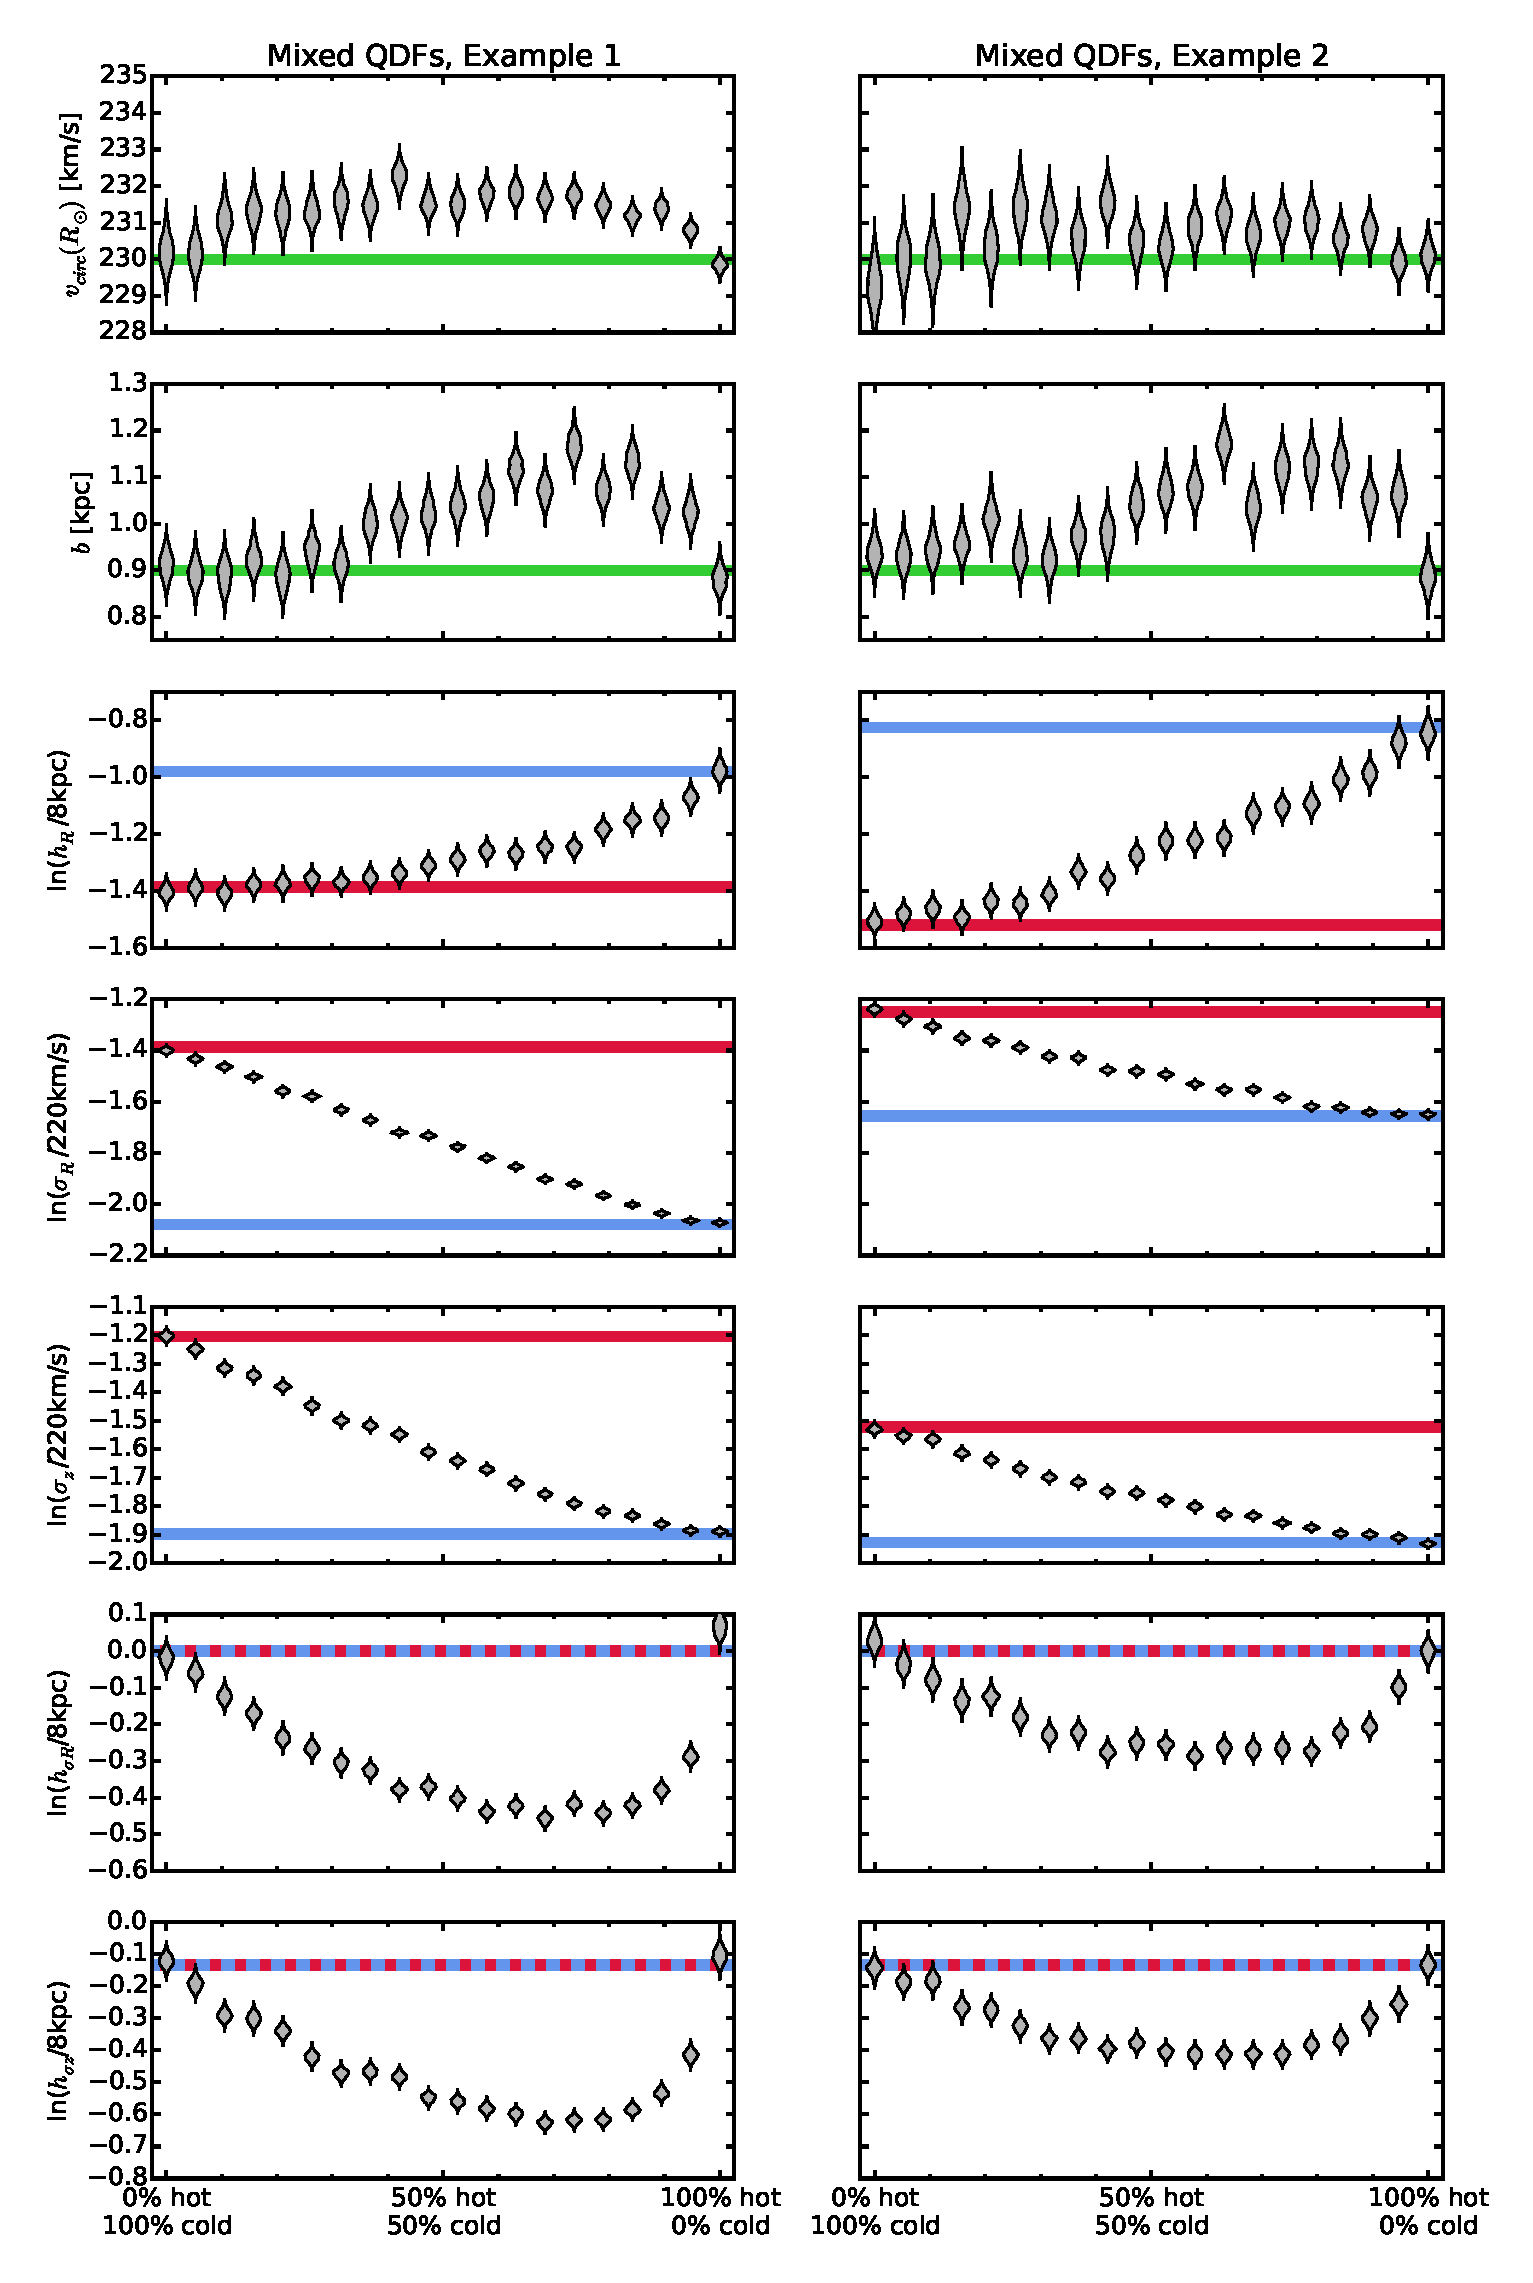
\includegraphics[width=0.8\textwidth]{figs/isoSphFlexMixCont_violins.eps}
\caption{The dependence of the parameter recovery on degree of pollution and temperature of the stellar population. To model the pollution of a hot stellar population by stars coming from a cool population and vice versa, we mix varying amounts of stars from two very different populations, as indicated on the $X$-axis. The composite mock data set is then fit with one single qDF. The violins represent the marginalized likelihoods found from the MCMC analysis. \emph{Example 1a} (\emph{Example 1b}) in the left (right) panels mixes the \texttt{hot} (\texttt{cool}) \MAP{} with the \texttt{cooler} (\texttt{hotter}) \MAP{} in Table \ref{tbl:referenceMAPs}. All model parameters used to create the mock data are given in Test \ref{test:isoSphFlexMix}, \emph{Example 1a) \& b)} in Table \ref{tbl:tests}. Some mock data sets are shown in Figure \ref{fig:isoSphFlexMix_mockdata_residuals}, first two rows, in the same colors as the violins here.  We find that a hot population is much less affected by pollution with stars from a cooler population than vice versa. \Wilma{[TO DO: rename $h_{\sigma R}$ to $h_{\sigma,R}$, $\sigma_R$ to $\sigma_{R,0}$ and analogous for $z$] [TO DO: Potential and/or population names in typewriter font] [TO DO: Comment from Jo: I feel like just showing one of these examples might be clearer, because they essentially demonstrate the same thing.] [TO DO: Remove $\sigma_R$ and $h_{\sigma,R}$ panels. Then make two columns with only one expample, potential and DF parameters separately]}}
\label{fig:isoSphFlexMixCont}
\end{figure*}



%FIGURE: isoSphFlexMixDiff

\begin{figure*}
\centering
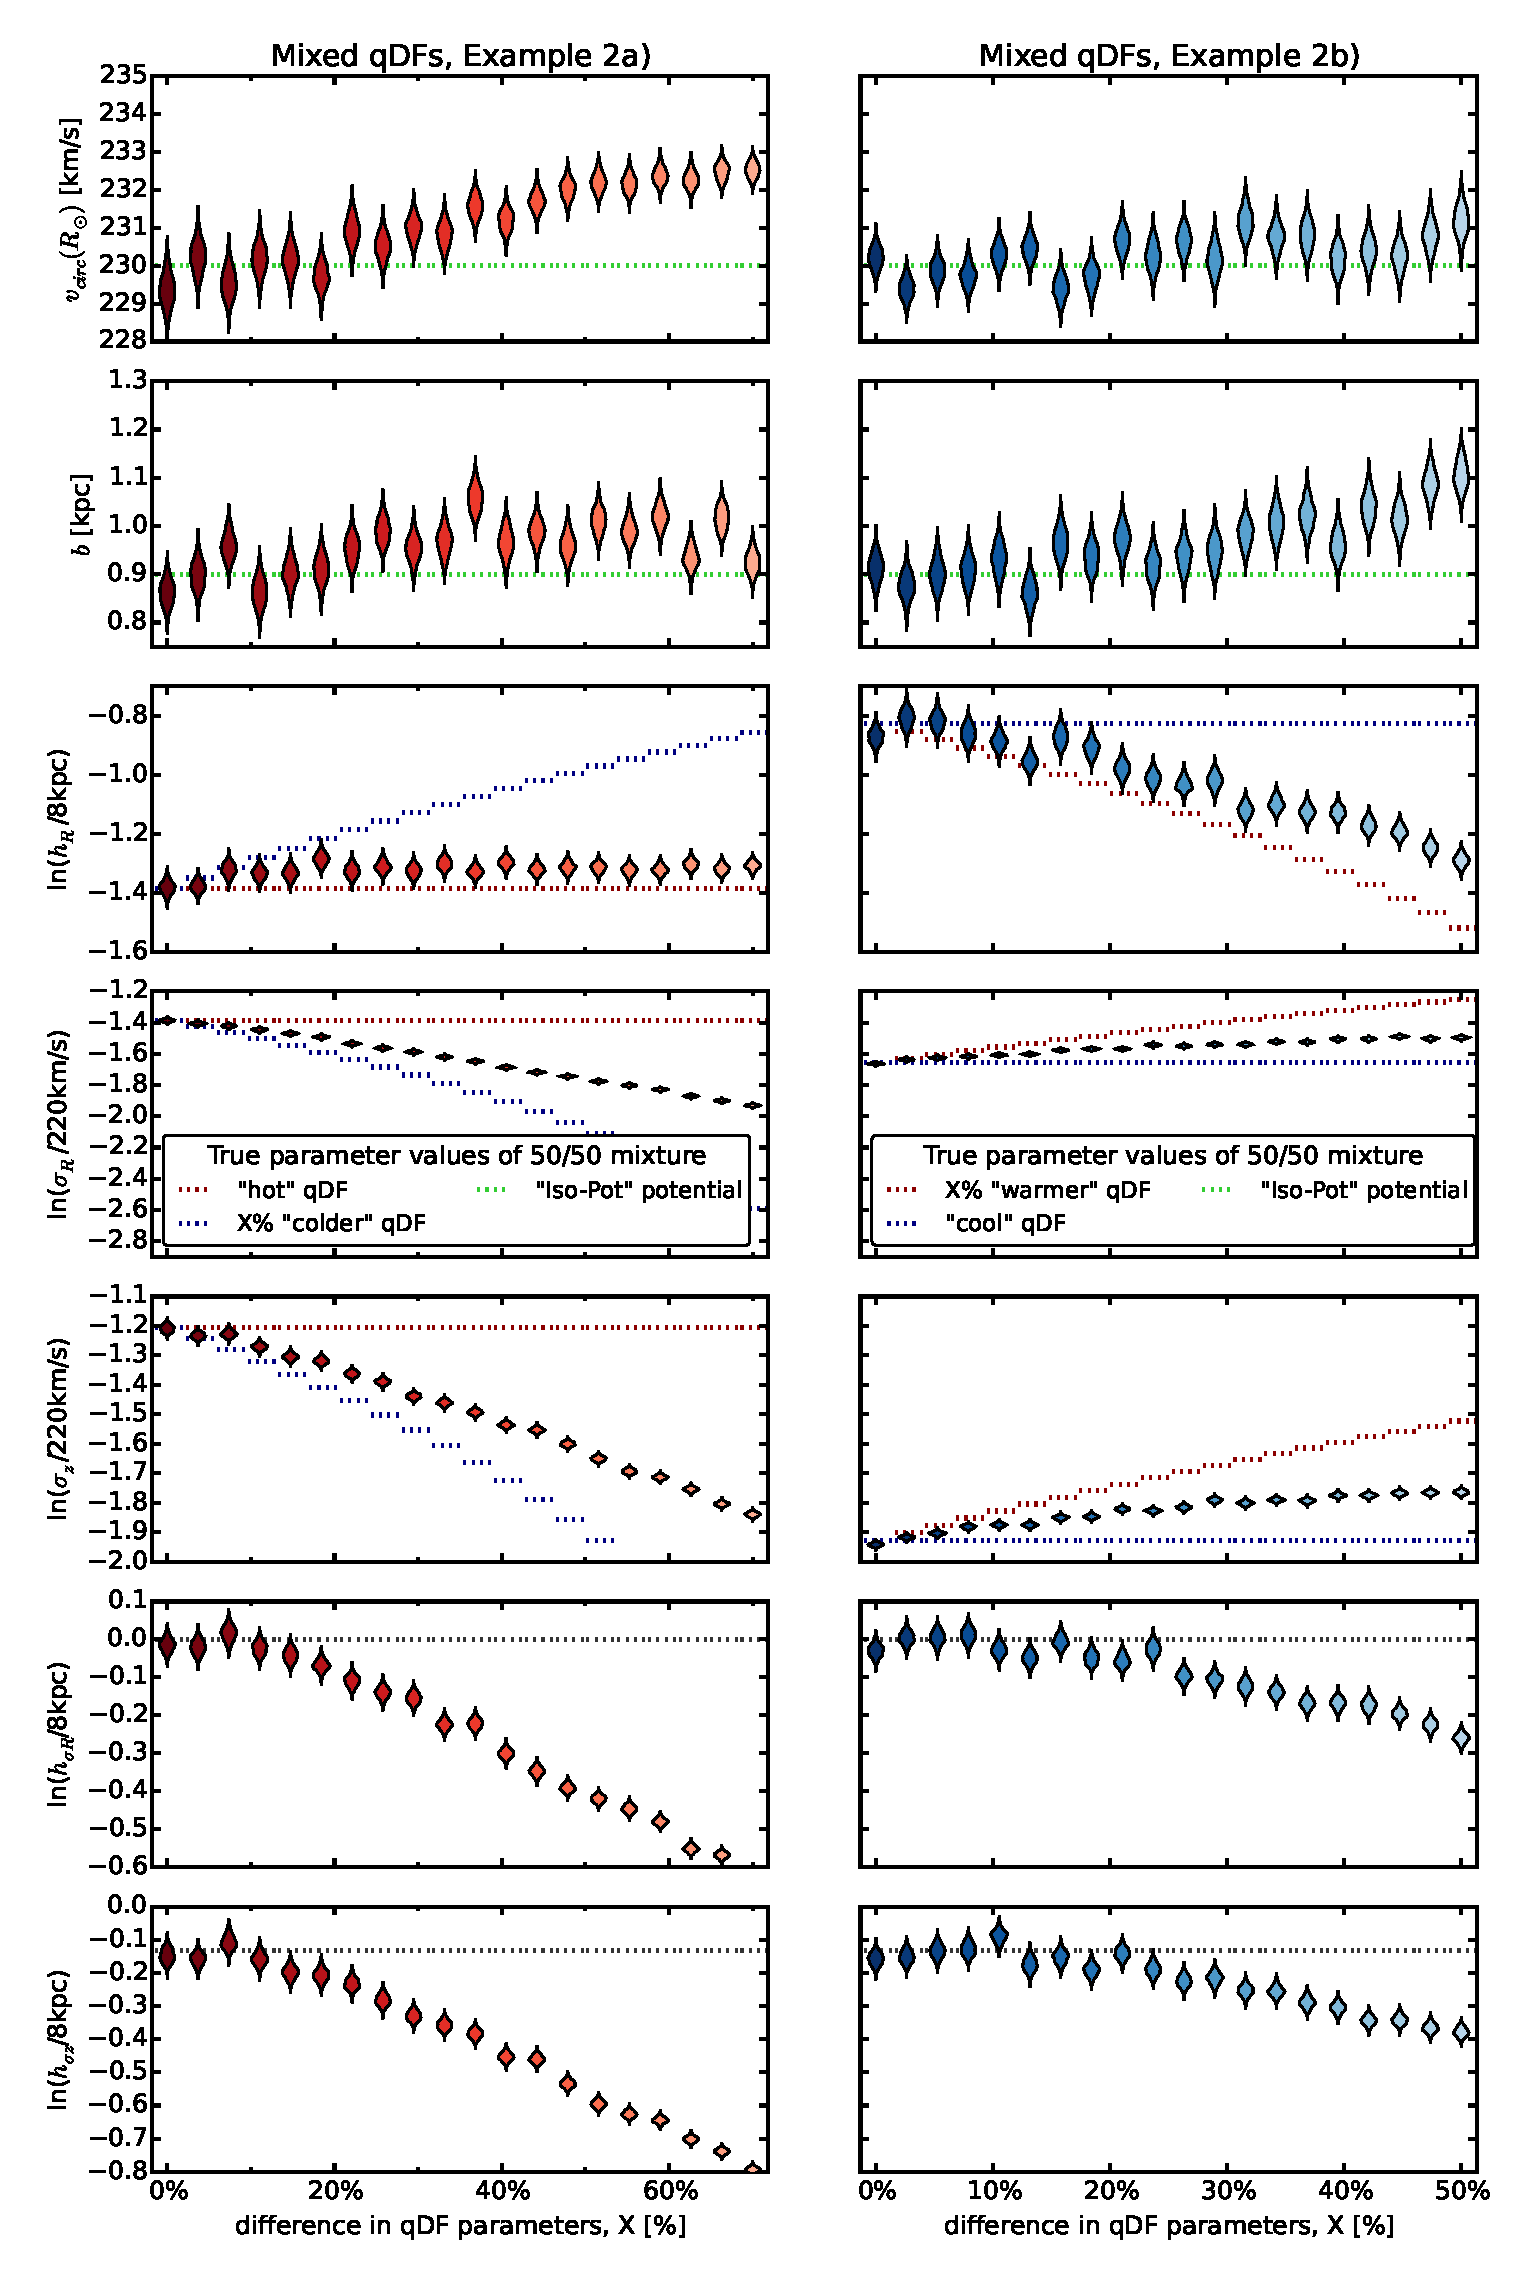
\includegraphics[width=0.8\textwidth]{figs/isoSphFlexMixDiff_violins.eps}
\caption{(Caption on next page.)}
\end{figure*}


\addtocounter{figure}{-1}
\begin{figure*} [t!]
\caption{The dependence of the parameter recovery on the difference in qDF parameters of a 50\%/50\% mixture of two stellar populations and their temperature. Half of the star in each mock data set in \emph{Example 2a} (\emph{Example 2b}) was drawn from the \texttt{hot} (\texttt{cool}) qDF in Table \ref{tbl:referenceMAPs}, and the other half drawn from a \texttt{colder} (\texttt{warmer}) population that has $X\%$ smaller (larger) $\sigma_{R,0}$ and $\sigma_{z,0}$ and $X\%$ larger (smaller) $h_R$. Each composite mock data set is then fitted by a single qDF and the marginalized MCMC likelihoods for the best fit parameters are shown as violins. The model parameters used for the mock data creation are given as Test \ref{test:isoSphFlexMix}, \emph{Example 2a) \& b)} in Table \ref{tbl:tests}. Some mock data sets are shown in figure \ref{fig:isoSphFlexMix_mockdata_residuals}, last two rows, where the distributions have the same colors as the corresponding best fit violins here. By mixing \MAPs{} with varying difference in their qDF parameters, we model the effect of bin size in the [Fe/H]-[$\alpha$/Fe] plane when sorting stars into different \MAPs{}: The smaller the bin size, the smaller the difference in qDF parameters of stars in the same bin. We find that the bin sizes should be chosen such that the difference in qDF parameters between neighbouring \MAPs{} is less than 20\%. [TO DO: rename $h_{\sigma R}$ to $h_{\sigma,R}$, $\sigma_R$ to $\sigma_{R,0}$ and analogous for $z$] [TO DO: Potential and/or population names in typewriter font]} 
\label{fig:isoSphFlexMixDiff}
\end{figure*}

%====================================================================

%\subsection{The Implications of Assuming a Potential Model which Differs from the Real Potential} \label{sec:results_potential}

%Motivation for the Test

We inspect if we can give constraints on the true potential, if our beliefs about the overall parametric form of the MW's potential are slightly wrong. We ignore deviations from axisymmetry and focus on a test case where the mock data was drawn from one axisymmetric potential (\texttt{MW14-Pot}) and is then analysed using another axisymmetric potential family (\texttt{KKS-Pot}), that does \emph{not} incorporate the true potential (compare the second and fourth panel in Figure \ref{fig:ref_pots}). In the analysis we assume the circular velocity at the sun to be fixed and known and only fit the parametric potential form. The results are shown in Figure \ref{fig:MW14vsKKS2SphFlex}.




%Results on the potential

The reference potential parameters of the \texttt{KKS-Pot} in Table \ref{tbl:referencepotentials} were found by adjusting the 2-component Kuzmin-Kutuzov St\"{a}ckel potential by \citet{bat94} such that it generates radial and vertical force profiles similar to the \texttt{MW14-Pot} from \citet{bov15} (dotted gray lines in Figure \ref{fig:MW14vsKKS2SphFlex}). The analysis results from \RM{} shown in Figure \ref{fig:MW14vsKKS2SphFlex}, red for a \texttt{hot} mock data \MAP{} and blue for a \texttt{cool} \MAP{}, give an comparable good or even better agreement with the true potential than the (by-eye) fit directly to the potential: especially the force contours, to which the orbits are sensitive, and the rotation curve are very tightly constrained and reproduce the true potential even outside of the observed volume of the mock tracers. This demonstrates that \RM{} provides an optimal best fit potential within the capabilities of the parametric potential model.
\\The density contours are less tightly constrained than the forces, but we still capture the essentials: The \texttt{hot} \MAP{} from Table \ref{tbl:referenceMAPs} constrains the halo; especially at smaller radii it is equally good or better than the \texttt{cool} \MAP{}. The \texttt{cool} \MAP{} gives tighter constraints on the halo in the outer region and recovers the disk better than the \texttt{hot} \MAP{}. This is in concordance with expectations as the \texttt{cool} \MAP{} has a longer tracer scale length and is more confined to the disk than the \texttt{hot} \MAP{} and therefore also probes the Galaxy in these regions better.
\\Overall the best fit disk is less dens in the midplane than the true disk. 

%Results on the qDF

Figure \ref{fig:MW14vsKKS2SphFlex_violins} compares the true qDF parameters with the best fit parameters. While tracer scale length and radial velocity dispersion profile are very well recovered, we misjudge the radial profile of the vertical velocity dispersion: $\sigma_{0,z}$ [TO DO: consistent] and $h_{\sigma,z}$ are both underestimated, which leads to a steeper profile and a lower dispersion around the sun. This is a direct result of the surface density underestimation in the midplane, the corresponding lower vertical forces around the sun (see also Figure \ref{fig:MW14vsKKS2SphFlex}) and therefore lower vertical actions [TO DO: I have honestly no idea, if this is a proper explanation. In configuration space both models, original mock data set and best fit, have exactly the same radial dispersion and velocity profile.]. Figure \ref{fig:MW14vsKKS2SphFlex_mockdata_residuals} demonstrates that even though the misjudgment of the potential lead to biases in the qDF parameters, the model is still a very good fit to the data.







%====================================================================

\begin{figure*}
\plotone{figs/MW14vsKKS2SphFlex_contours_compare.eps}
\caption{Recovery of the gravitational potential if the assumed potential model (\texttt{KKS-Pot} with fixed $v_\text{circ}(R_\odot)$) and the true potential of the (mock) stars (\texttt{MW14-Pot} in Table \ref{tbl:referencepotentials}) is slightly different. We show the circular velocity curve, as well as contours of equal density, radial and vertical force in the $R$-$z$-plane, and compare the true potential with 50 [TO DO: CHECK] sample potentials drawn from the posterior distribution function found with the MCMC for a \texttt{hot} (red) and a \texttt{cool} \MAP{} (blue). All model parameters are given as Test \ref{test:MW14vsKKS2SphFlex} in Table \ref{tbl:tests}. [TO DO: Do more analyses???] [TO DO: fancybox Legend] [TO DO: Potential and/or population names in typewriter font] [TO DO: Reference correct Table in Plot]}
\label{fig:MW14vsKKS2SphFlex}
\end{figure*}

\begin{figure*}
\plotone{figs/MW14vsKKS2SphFlex_violins.eps}
\caption{Recovery of the qDF parameters for the case where the true and assumed potential deviate from each other (Test \ref{test:MW14vsKKS2SphFlex} in Table \ref{tbl:tests}). The thick red (blue) lines represent the true qDF parameters of the \texttt{hot} (\texttt{cool}) qDF in Table \ref{tbl:referenceMAPs} used to create the mock data, surrounded by a 10\% error region. The grey violins are the marginalized likelihoods for the qDF parameters found simultaneously with the potential constraints shown in Figure \ref{fig:MW14vsKKS2SphFlex}. [TO DO: rename $h_{\sigma R}$ to $h_{\sigma,R}$, $\sigma_R$ to $\sigma_{R,0}$ and analogous for $z$]}
\label{fig:MW14vsKKS2SphFlex_violins}
\end{figure*}

\begin{figure*}
\plotone{figs/MW14vsKKS2SphFlex_mockdata_residuals.eps}
\caption{Comparison of the distribution of mock data in configuration space created in the \texttt{MW14-Pot} potential (solid lines) with a \texttt{hot} (red) and \texttt{cool} (blue) \MAP{} (Test \ref{test:MW14vsKKS2SphFlex} in Table \ref{tbl:tests}), and the best fit distribution using a \texttt{KKS-Pot} potential (dashed lines). The best fit potentials are shown in Figure \ref{fig:MW14vsKKS2SphFlex} and the corresponding best fit qDF parameters in Figure \ref{fig:MW14vsKKS2SphFlex_violins}. The best fit [TO DO: Continue Caption] [TO DO: Potential and/or population names in typewriter font]}
\label{fig:MW14vsKKS2SphFlex_mockdata_residuals}
\end{figure*}



%====================================================================





%%-----------------------------------------------------------------------------------------------------------------------------------------------------------------------------
%
%%-----------------------------------------------------------------------------------------------------------------------------------------------------------------------------
%%Discussion etc.
%\section{Discussion and Summary} \label{sec:discussionsummary}

Recently implementations of action DF - based modelling of 6D data in the Galactic disk have been put forth, in part to lay the ground-work fo Gaia \citep{bov13,2013MNRAS.433.1411M,pif14,san15}.
 
 We present \RM, an improved implementation of the dynamical modelling machinery by \citet{bov13}, to recover the potential and orbit distribution function of stellar \MAPs{} within the Galactic disk. In this work we investigated the capabilities, strengths and weaknesses of \RM by testing its robustness against the breakdown of some of its assumptions - for well defined, isolated test cases using mock data. Overall the method works very well and reliable, also if there are small deviations of the model assumptions from the real world galaxy.

\subsection{Improved Computational Speed for Application to Larger Data Sets}

\RM applies a full likelihood analysis and is statistically well-behaved. It allows for a straightforward implementation of different potential model families and a flexible number of free fit parameters in potential and qDF. It also accounts for selection effects by using full 3D selection functions (given some symmetries). \RM is an asymptotically normal, un-biased estimator and the precision of parameter recovery increases by $1/\sqrt{N}$ with the number of stars.\\

Large data sets in the age of Gaia require more, and more accurate, likelihood evaluations for more flexible models. To be able to deal with these increased computational demands and explore larger parameter spaces, we sped up the code by combining a nested grid approach with MCMC and by faster action calculation using the St\"{a}ckel \citep{bin12} interpolation grid by \citet{bov15}. Especially accurately determining the likelihood normalisation will be of crucial importance for large data sets. The nested-grid approach automatizes the search for the optimal normalisation integration ranges (\emph{fiducial} qDF) and start position for the MCMC walkers, which helps the MCMC to converge fast and to reduce biases due to insufficient accuracy. However, application of \RM to millions of stars simultaneously with acceptable accuracy will still be a task for supercomputers and calls for even more improvements and speed-up in the fitting machinery.

\subsection{Modelling Sensitivity to Properties and Unaccounted Imperfections of the Data Set}

\paragraph{Choice of observation volume.} We found that the \emph{position} of the survey volume maters little, in the sense that there are no regions in the Galaxy that contain intrinsically stars on manifestly more diagnostic orbits than others. Closer to the disk and at smaller Galactocentric radii it is only the increased number of stars that will lead to tighter constraints. Concerning the \emph{shape} of the survey volume, a large radial \emph{and} vertical coverage is best. In the axisymmetric case phi coverage doesn't matter. Making a volume cut for stars, that lie around $R_\odot$ but at larger $phi$, could therefore improve the results, if their measurements are very uncertain.
\\\MAPs{} of different scale length and temperature probe different regions of the Galaxy \citep{bov13}. But there is no easy rule of thumb for which survey volume and stellar population which potential and DF parameter is constrained best.

\paragraph{Selection function misjudgment.} Surprisingly \RM seems to be very robust against misjudgments in the selection function of the data. The reason for this robustness could be, that missing stars in the data set do not affect the connection between a star's velocity and position, which is given by the potential. A lot of information about the potential profile is stored in the rotation curve - but even when not including measurements of tangential velocities in the analysis, small misjudgments of the incompleteness do not affect the potential recovery.
\\That we reproduce the qDF equally well, could be due to the symmetry of our assumed incompleteness profiles around the sun. We investigated a decrease in knowledge of the data completeness in distance from the sun and Galactic plane. Our test with the radial incompleteness profile could be understood as a decreasing detection rate due to the lower apparent brightness of stars at larger distances. The test with the planar incompleteness profile could mimic a misjudgment of the dust obscuration within the Galactic plane. Both effects would show the same symmetries as tested in this work. 
\\This result is encouraging for future studies, but nevertheless surprising as it was previous believed that knowing the (spatial) selection function very precisely is of large importance for dynamical modelling \citep{rix13}.

\paragraph{Measurement errors.} Properly convolving the likelihood with measurement errors is computational very expensive. By ignoring positional errors and only including distance errors as part of the velocity error, we can drastically reduce the computational costs. For stars within 3 kpc from the sun this approximation works well for distance errors of $\sim 10\%$ or smaller. The number of MC samples needed for the error convolution using MC integration scales by $N_\text{error} \propto (\delta v_\text{max})^2$ with the maximum velocity error at the edge of the sample. If we did not know the true size of the proper motion measurement errors perfectly, we can only reproduce the true model parameters to within $\lesssim 2$ sigma [TO DO: Can I say sigma???] [TO DO: Check???] as long as we do not underestimate it by more than $10\%$ and for proper motion errors $\lesssim 2 \text{ mas yr}^{-1}$.

\subsection{Data Deviations from the Modelling Assumptions about the Distribution Function and the Potential}

\paragraph{Deviations from the qDF Assumption.}  Our modelling is founded on the assumption, that we can identify {\sl a priori} sub-components of the Galactic disk that follow a qDF (e.g. by considering \MAPs{}). There are two reasons why any chosen sub-sample of star (here a \MAP{}) may not be well described by any qDF. Either, because nature is more complex, or because even if perfect
\MAPs{} would be well described by qDFs finite abundance errors would mix \MAPs{}.  We have considered both cases.

 In Example 1 in \S\ref{sec:results_mixedDFs} we investigated how well we can recover the potential, if this assumption was not perfectly satisfied, i.e. the \MAPs{} true DF does not perfectly follow a qDF. We considered two cases: a) a hot DF, that has less stars at small radii and more stars with low velocities than predicted by the qDF (reddish data sets in Figure \ref{fig:isoSphFlexMix_mockdata_residuals}), or b) a cool DF that has broader velocity dispersion wings and less stars at large radii than predicted by the qDF (bluish data sets). We find that case a) would give more reliable results for the potential parameter recovery.
\\If we assumed that the distribution of stars from one \MAP{} is caused by radial migration away from the initial location of star formation, it would more likely that the qDF overestimates the true number of stars at smaller radii than underestimating it at larger radii. [TO DO: Is this actually a sensible argument???]
\\Following this, focusing the analysis especially on hotter \MAPs{} could be an advisable way to go in the future, if there is doubt that the stars truly follow the qDF.

 Another critical point is the binning of stars into \MAPs{} depending on their metallicity and $\alpha$ abundances. Example 2 in \S\ref{sec:results_mixedDFs} could be understood as a model scenario for decreasing bin sizes in the metallicity-$\alpha$ plane when sorting stars in different \MAPs{}, assuming that there is a smooth variation of qDF within the metallicity-$\alpha$ plane and each \MAP{} indeed follows a qDF. We find that, in the case of 20,000 stars in each bin, differences of $20\%$ in the qDF parameters of two neighbouring bins can still give quite good constraints on the potential parameters. 
\\We compare this with the relative difference in the qDF parameters in the bins in Figure 6 of \cite{bov13}, which have sizes of $[Fe/H] = 0.1$ dex and $\Delta [\alpha/Fe] = 0.05$ dex. It seems that these bin sizes are large enough to make sure that $\sigma_{R,0}$ and $\sigma_{z,0}$ of neighbouring \MAPs{} do not differ more than $20\%$. Figure \ref{fig:isoSphFlexMixCont} and \ref{fig:isoSphFlexMixDiff} suggest that especially the tracer scale length $h_R$ needs to be recovered to get the potential right. For this parameter however the bin sizes in Figure 6 of \cite{bov13} might not yet be small enough to ensure no more than $20\%$ of difference in neighbouring $h_R$. This is especially the case in the low-$\alpha$ ($[\alpha/Fe] \lesssim 0.2$), intermediate-metallicity ($[Fe/H] \sim -0.5$) \MAPs{}. The above is valid for 20,000 stars per \MAP{}. In case there are less than 20,000 stars in each bin the constraints are less tight and due to Poisson noise one could also allow larger differences in neighbouring \MAPs{} while still getting reliable results.

\paragraph{Gravitational Potential beyond the Parameterized Functions Considered.}  In the long run \RM should incorporate a family of gravitational potential models that can reproduce the essential features of the MW's true mass distribution. While our fundamental assumption of the Galaxy's axisymmetry is at odds with the obvious existence of non-axisymmetries in the MW, we will not dive into investigating this implications in the scope of this paper. Instead we test how a misjudgment of the parametric potential form affects the recovery by fitting a potential of St\"{a}ckel form \citep{bat94} to mock data from a different potential family with halo, bulge and exponential disk. The recovery is quite successful and we get the best fit within the limits of the model. However, even a strongly flattened St\"{a}ckel potential component has difficulties to recover the very flattened mass distribution of an exponential disk. This leads to misjudgment of the qDF parameters describing the vertical action distribution, $\sigma_{z,0}$ and $h_{\sigma,z}$. As the qDF parameter $\sigma_{z,0}$ corresponds to the physical vertical velocity dispersion at the sun, a comparison with direct measurements could be a valuable cross-checking reference. [TO DO: This might not be true. For isochrone and Staeckel potential I get this behaviour, but not for the MW14-Pot!!! Might be, because it's not separable??? Check!!!] In case of as many as 20,000 stars we should therefore already be able to distinguish between different potential models.
\\The advantage of using a St\"{a}ckel potential with \RM is firstly the exact and fast action calculation via the numerical evaluation of a single integral, and secondly that the potential has a simple analytic form, which greatly speeds up calculations of forces and frequencies (as compared to potentials in which only the density has an easy description like the exponential disk). A superposition of several simple Kuzmin-Kutuzov St\"{a}ckel components can successfully produce MW-like rotation curves (see \citet{bat94}, \citet{2003MNRAS.340..752F} and Figure \ref{fig:MW14vsKKS2SphFlex}) and one could think of adding even more components for more flexibility, e.g. a small roundish component for the bulge.
\\The potential model used by \citet{bov13} had only two free parameters (disk scale lentgh and halo contribution to $v_\text{circ}(R_\odot)$. To circumvent the obvious disadvantage of this being at all not flexible enough, they fitted the potential separately for each \MAP{} and recovered the mass distribution for each \MAP{} only at that radius for which it was best constrained - assuming that \MAPs{} of different scale length would probe different regions of the Galaxy best. Based on our results in Figure \ref{fig:MW14vsKKS2SphFlex} this seems to be indeed a sensible approach [TO DO: Check that this is indeed the case - it is not clear to me from the plot. ???].
\\We suggest that combining the flexibility and computational advantages of a superposition of several St\"{a}ckel potential components with probing the potential in different regions with different \MAPs{} as done by \citet{bov13}, could be a promising approach to get the best possible constraints on the MW's potential.

\subsection{Different Modelling Approaches using Action-based Distribution Functions}

We have focussed for the time being on \MAPs{} for a number of reasons: First, they seem to permit simple DFs \citep{bov12b,bov12c,bov12d}, i.e. approximately qDFs \citep{tin13}. Second, all stars, e.g. those from different \MAPs{}, must orbit in the same potential. Therefore each \MAP{} will and can yield quite different DF parameters; but each \MAP{} will also provide a (statistically) independent estimate of the potential parameters. At the same time -- if all is well -- those potential parameters, derived from different \MAPs{}, should be mutually consistent. In some sense, this approach focusses on constraining the potential, treating the DF parameters as nuisance parameters.

The main drawback is that we have many astophysical reasons that the DF properties (for reasons of galaxy evolution and chemical evolution) are astrophysically linked between different \MAPs{}. Ultimately, the goal is to do a fully consistent chemodynamical model that simultaneously fits the potential and $\text{DF}(\vect{J},\text{[X/H]})$ simultaneously (where [X/Fe] denotes the full abundance space) with a full likelihood analysis. 
\\This has not yet been attempted. 

Since the first application of \RM by \citet{bov13} there have been two similar efforts to constrain the Galactic potential and/or orbit distribution using action-based distribution functions:

\citet{pif14} fitted both potential and a $f(\vect{J})$ to giant stars from the RAVE survey \citep{ste06} and the vertical stellar number density profiles in the disk by \citet{jur08}. They did not include any chemical abundances in the modelling. Instead, they used a superposition of action-based DFs to describe the overall stellar distribution at once: a superposition of qDFs for cohorts in the thin disk, a single qDF [TO DO: CHECK] for the thick disk stars and an additional DF for the halo stars. Taking proper care of the selection function requires a full likelihood analysis and the calculation of the likelihood normalisation is computational expensive. \citet{pif14} choose to circumvent this problem by directly fitting a) histograms of the three velocity components in eight spatial bins to the velocity distribution predicted by the DF and b) the vertical density profile predicted by the DF to the profiles by \citet{jur08}. The vertical force profile of their best fit mass model nicely agrees with the results from \citet{bov13} for $R>6.6$ kpc. The disadvantage of their approach is, that by binning the stars spatially, a lot of stellar information is not used.

\citet{san15} have focussed on understanding the abundance-dependence of the DF, relying on a fiducial potential. They developed extended distribution functions, i.e. functions of both actions and metallicity for a superposition of thin and thisk disk, each consisting of several cohorts described by qDFs, a DF for the halo, a functional form of the metallicity of the interstellar medium at the time of birth, and a simple prescription for radial migration. They applied a full likelihood analysis accounting for selection effects and found a best fit for the eDF in a fixed fiducial potential by \citet{deh98} to the stellar phase-space and metallicity [TO DO: CHECK] data of the Geneva-Kopenhagen Survey (GS) \citep{2004A&A...418..989N,2009A&A...501..941H} and the stellar density curves by \citet{{gil83}}. Their best fit predicted the velocity distribution of SEGUE G dwarfs quite well, but had biases in the metallicity distribution, which they accounted to being a problem with the SEGUE metallcities. 

\subsection{On the Assumption of Axisymmetry}

The key assumption in our modelling, as well as in the approaches by \citet{pif14} and \citet{san15} described above, is the overall axisymmetry of Galaxy's potential and DF. This has the convenient advantage, that actions are conserved in axisymmetric potentials and can be calculated straightforward via the \emph{St\"{a}ckel Fudge} by \citet{bin12} and/or a single integration (in the case of separable potentials). Of course the Galactic disk is in reality not axisymmetric and actions are not conserved: Spiral arms in the disk and the Galactic bar lead to angular momentum exchange and therefore radial migration of stars, i.e. the orbit on which the stars were born on are modified \citep{2011A&A...527A.147M,2014MNRAS.443.2757K}. Apart from these obvious non-axisymmetries in the Galaxy, the disk itself is not smooth, as there is lot of sub-structure, streams and moving groups within the disk. A famous example is the Arcturus moving group, for which \citet{2004ApJ...601L..43N} found that the stars might have their origin in a disrupted satellite.
\\Spiral arms, the stirring of the Galactic bar and the disk sub-structure will undoubtedly affect our modelling with \RM. How strong this effect will be and if the modelling can still work, needs to be investigated in detail in future work, e.g. by trying to recover the potential in N-body simulations. But as actions are conserved under adiabatic changes of the potential \citet{bin08}, and the vertical action under radial migration [TO DO: REF], there is some hope, that the modelling could still work.

The ultimate goal would be to theoretically describe those non-axisymmetries and sub-structures in terms of DFs in action/angle-abundance space. We see the current axisymmetric modelling approaches as intermediate step to this goal: \citet{1998AJ....115.2384D} described the disk's overall stellar distribution as a smooth background distribution superimposed with sub-structure; the axisymmetric DFs used and to be found by \RM and similar approaches could be treated as this smooth background. Firstly, this smooth background DF could help to actually find and identify the disk substructure in action space (see e.g. \citet{2010MNRAS.409..145S,2008ApJ...685..261K} for similar approaches to find disk substructure, which then helps to find DF descriptions. Secondly, and because simple superposition of action-based DFs is possible (see e.g. [TO DO: REF (see Payel's hint)]), the substructure DFs could then be directly added to the background DF and incorporated in the modelling. In other words, modelling the Galaxy together with its non-axisymmetries and substructure could be approached as applying perturbations to an axisymmetric equilibrium model. And \RM will help finding this equilibrium model.

Such a Galaxy model will be also important in the meantime: Many studies of Galaxy structure and evolution use orbits as tracers and therefore require a reliable fiducial potentials to turn stellar positions and velocities into orbits. And as long as we are as far away from realistic Galaxy models as we are now, the axisymmetric case well need to be our reference.
%\section{Acknowledgments}

[TO DO]

The authors thank Glenn van de Ven for the idea of using Kuzmin-Kutuzov St\"{a}ckel potentials in this case study.
%%-----------------------------------------------------------------------------------------------------------------------------------------------------------------------------
%
\begin{appendix}
\subsection{Influence of wrong assumptions about incompleteness of the data parallel to the Galactic plane} \label{sec:incompZ}

In \S\ref{sec:results_incompR} we found a striking robustness of the \RM modelling approach against wrong assumptions about the radial incompleteness of the data set. To further test this result, we investigate a different completeness function that drops with distance from the Galactic plane (see Test \ref{test:isoSphFlexIncomp}, Example 2, in Table \ref{tbl:tests} and Figure \ref{fig:isoSphFlexIncompZ_mockdata}). We get a similar robust behaviour for small deviations, and only slightly less robustness for larger deviations. That an explanation for this robustness could be, that a lot of information about the potential comes from the rotation curve, which is not affected by incompleteness, is demonstrated in Figure \ref{fig:isoSphFlexIncomp_marginal_violins}.

\paragraph{Marginalization over $v_T$.} The likelihood in Equation \ref{eq:prob} is marginalized over the coordinate $v_T$ as follows
\begin{eqnarray*}
&&\left. \mathscr{L}(\pmodel \mid D)\right|_\text{($v_T$ marg.)}\\
&=& \prod_i^N P_\text{($v_T$ marg.)} (\vect{x}_i,v_{R,i},v_{z,i} \mid \pmodel)\\
&\equiv& \prod_i^N v_0 \cdot \int_0^{1.5v_\text{circ}(R_\odot)} \diff v_T \ P(\vect{x}_i,v_{R,i},v_{T},v_{z,i} \mid \pmodel )
\end{eqnarray*}
where $P(\vect{x},\vect{v} \mid \pmodel)$ is the same as in Equation \ref{eq:prob} and the numerical integral over $v_T$ is performed as a 24th order Gauss-Legendre quadrature. The additional factor of $v_0$ is needed to get the units of $P_\text{($v_T$ marg.)} (\vect{x}_i,v_{R,i},v_{z,i} \mid \pmodel)$ right.

%FIGURE:  isoSphFlexIncompZ
\begin{figure}
\centering
\begin{minipage}{.48\textwidth}
  \centering
\includegraphics[width=0.8\textwidth]{figs/isoSphFlexIncompZ_mockdata.eps}
\caption{Selection function and mock data distribution for investigating vertical incompleteness of the data. All model parameters are summarized as Test \ref{test:isoSphFlexIncomp}, Example 2, in Table \ref{tbl:tests}. The survey volume is a sphere around the sun and the percentage of observed stars is decreasing linearly with distance from the Galactic plane, as demonstrated in the left panel. How fast this detection/incompleteness rate drops is quantized by the factor $\epsilon_z$. Histograms for four data sets, drawn from two \MAPs{} (\texttt{hot} in red and \texttt{cool} in blue, see Table \ref{tbl:referenceMAPs}) and with two different $\epsilon_z$, 0 and 0.7, are shown in the right panel for illustration purposes. \Wilma{[TO DO: Potential and/or population names in typewriter font]}} 
\label{fig:isoSphFlexIncompZ_mockdata}
\end{minipage}%
\begin{minipage}{.48\textwidth}
  \centering
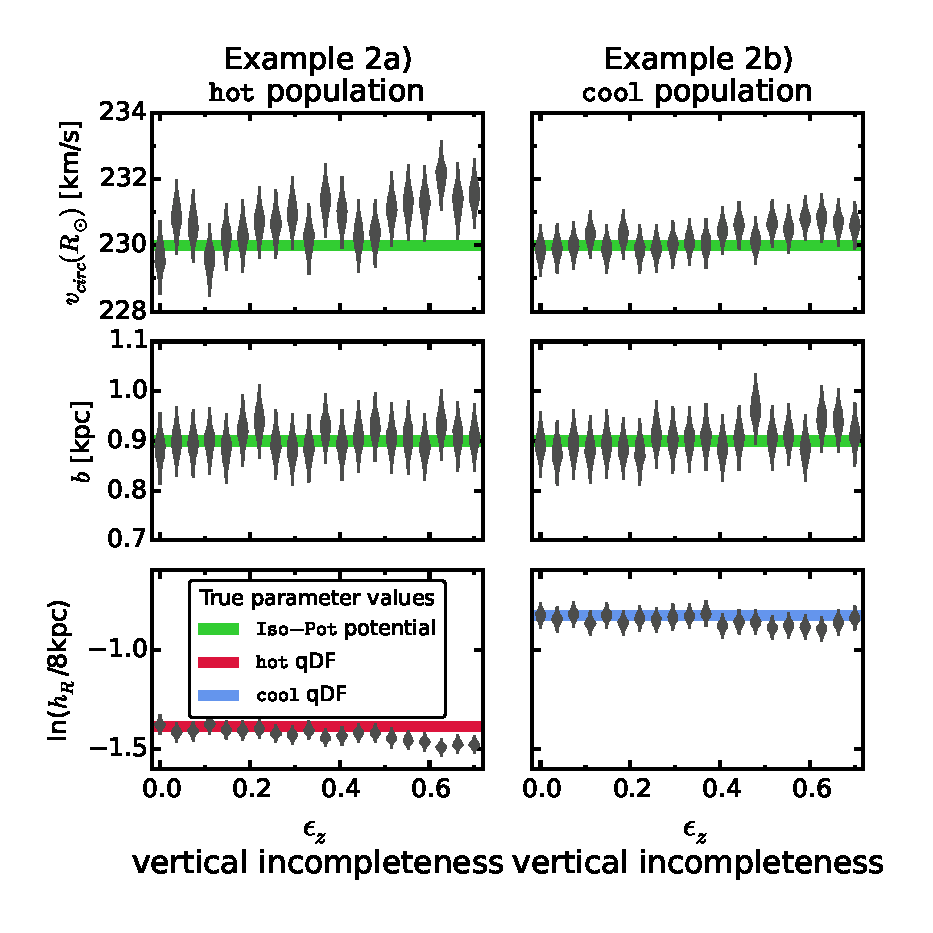
\includegraphics[width=0.8\textwidth]{figs/isoSphFlexIncompZ_violins_2.eps}
\caption{Influence of wrong assumptions about the incompleteness parallel to the Galactic plane of the data on the parameter reocovery with \RM{}. Each mock data set was created having different incompleteness parameters $\epsilon_z$ (shown on the $x$-axis and illustrated in Figure \ref{fig:isoSphFlexIncompZ_mockdata}) and the model parameters are given as Test \ref{test:isoSphFlexIncomp}, Example 2, in Table \ref{tbl:tests}. The analysis however didn't know about the incompleteness and assumed that all data sets had constant completeness within the survey volume ($\epsilon_z = 0$). The marginalized likelihoods from the fits are shown as violins. The green lines mark the true potential parameters (\texttt{Iso-Pot}) and the red and blue lines the true qDF parameters (\texttt{hot} \MAP{} in red and \texttt{cool} \MAP{} in blue), which we tried to recover. The \RM{} method seems to be robust against small to intermediate deviations between the true and the assumed vertical data incompleteness, as well as the radial incompleteness in Figure \ref{fig:isoSphFlexIncompZ_violins}.} 
\label{fig:isoSphFlexIncompZ_violins}
\end{minipage}
\end{figure}


\begin{figure*}
\plotone{figs/isoSphFlexIncomp_marginal_violins_2.eps}
\caption{Influence of wrong assumptions about radial and vertical incompleteness on the parameter recovery, when \emph{not} including information about the tangential velocities in the analysis. The mock data sets are the same as in Figure \ref{fig:isoSphFlexIncompR_violins} and \ref{fig:isoSphFlexIncompZ_violins}, but this time we did not include the data coordinates $v_T$ in the analysis and therefore marginalized the likelihood over $v_T$ instead (see \S\ref{sec:incompZ}). This demonstrates that a lot of information about the potential is actually stored in the rotation curve, i.e. $v_T(R)$, which is not affected by removing stars from the data set. But even if we do not include $v_T$ we can still recover the potential within the errors, at least for small ($\epsilon_z \lesssim 10\%$).} 
\label{fig:isoSphFlexIncomp_marginal_violins}
\end{figure*}

\Wilma{[TO DO: Mention in text or caption how the panels looked that I removed.]}
\end{appendix}
%
%\clearpage
%\section{Stuff that still needs to be done or thought about}

\paragraph{Questions that haven't been covered so far:}
\begin{itemize}
\item What happens, when the errors are not uniform?
\item What if errors in distance matter for selection?
\end{itemize}

\paragraph{Stuff that needs to be further examined in fig. \ref{fig:wedFlexVol_bias_vs_SE} about the survey volume:}
\begin{itemize}
\item[[TO DO]] Do we still get the same results, if we use an acceptable high numerical accuracy for the action grid?
\item[[TO DO]] Do the biases for the orange volume disappear, when we increase the integration range in vT?
\item[[TO DO]] Add the previous two volumes again, that had small extent in both R and z, or large extent in both.
\item[[TO DO]] Maybe add volume at smaller radius with large vertical extent?
\item[[TO DO]] Do we explicitely want to test, if it matters, if the radial coverage is larger or smaller the disk scale length, and the vertical coverage is larger or smaller than the disk scale height?
\end{itemize}

\paragraph{Stuff that needs to be further examined about the robustness against data incompleteness:}
\begin{itemize}
\item[[TO DO]] Maybe instead of decreasing completeness with height above the plane, a completeness
that INcreases with height above the plan, to model e.g. obscuration due to dust.
\item[[TO DO]] Make similar test as isoSphFlexIncompR, but with KKS potential, to test, if this
robustness is a special case for the isochrone potential.
\end{itemize}

\paragraph{General Stuff}
\begin{itemize}
\item[[TO DO:]] Rename everywhere $N_\text{sigma}$ to $n_\text{interval}$ or something like this.
\item[[TO DO:]] Look up what McMillan \& Binney 2013 have to say about the numerical accuracy of the normalisation. Sanders \& Binney (2015) are quoting them on that matter.
\item[[TO DO:]] Consistent capitals in section titles.
\item[[TO DO:]] Make consistent: use of $\sigma_R$ and $\sigma_{R,0}$ as profile or dispersion at sun. --> Done. But not yet in Figures.
\item[[TO DO:]] Make consistent $h_{\sigma_R}$ --> $h_{\sigma,R}$ --> Done. But not yet in Figures.
\item[[TO DO:]] Make consistent $M$ --> \pmodel
\item[[TO DO:]] Make consistent MAP --> \MAP
\item[[TO DO:]] Make consistent number of stars $N$ --> $N_\text{sample}$, introduce somewhere
\item[[TO DO:]]  introduce \pdf somewhere
\item[[TO DO:]]  Rename all cite in citet and citep
\item[[TO DO:]] Make a backslash before the year in all references.
\item[[TO DO:]] Make sure, MW, DF, qDF, pdf are somewhere written and introduced explicitely
\item[[TO DO:]] Find out, if the bibitem references should be the journal short cuts (e.g. to be able to be referenced on ADS)
\item[[TO DO:]] Make Legends in figures consistent. (fancybox)
\item[[TO DO:]] einheitlich, convolution of model probability with measurement errors, nicht deconvolution of likelihood
\item[[TO DO:]] einheitlich $\text{km s}^{-1}$ and $\text{mas yr}^{-1}$
\item[[TO DO:]] Make alpha and delta to $\text{RA}$ and $\text{DEC}$ everywhere
\item[[TO DO:]] Introduce Monte Carlo (MC) somewhere, and use MC everywhere else.
\item[[TO DO:]] Einheitlich Leerzeichen oder kein Leerzeichen zwischen Paragraph Symbol und Zahl.
\item[[TO DO:]] Should I give each equation a label or only those I'm referencing somwhere?
\item[[TO DO:]] Check that really everywhere fig. --> Figure, table --> Table, eq. --> Equation --> Done
\item[[TO DO:]] Make hyperref references for all tests. --> Done
\item[[TO DO:]] Make Staeckel fudge everywhere \emph{St\"{a}ckel Fudge}
\item[[TO DO:]] Make sure \MAP{} and \MAPs{} with brackets everywhere
\end{itemize}

%=====================================================

%15. May 2015 --> Meet with HW to write
%
%* just explain what the best solution in analysis section is, don't explain too much about other (worse) techniques
%* Numerical accuracy plot is a result
%* 20,000 stars --> much larger than current sample sizes (200 stars), but forecasting to larger sample sizes with Gaia (?)
%* Fig. 3,4,5 --> Behaviour in the limit of large samples
%* Change order of sections according to order in Results section intro
%* mention in introduction that we do not investigate axisymmetry
%* limit of lousy data --> model assumptions are not limiting. very good data --> model assumptions are limiting. Bovy & Rix: 150 stars per MAP. When we get larger samples sizes, the modelling will be limited by the model assumptions.
%* rename model parameters $M$ into $p_M$
%* mock data in action space plot --> in mock data section
%* accuracy plot --> in "Numerical accuracy of the likelihood calculation" section
%* in section on numerical accuracy erwähnen, dass wir in the limit of many stars aufpassen müssen, dass wir die normalisierung genau genug berechnen.
%* Macro fuer MAP schreiben: In Kapitälchen, damit klar ist, dass das ein Akronym ist
%* Citation korrigieren: bo13 --> bov13
%* Check how many stars were typically in a Bovy&Rix13 MAP
%* Triangle plot --> I talk about likelihood, but it is a pdf!
%* Priors: We want parameter estimates that alre tight enough, such that it does not matter, if we had assumed a flat or a logarithmically flat prior
%* Introduce somewhere the 20,000 stars 
%* if the priors are sufficiently flat, likelihood and pdf are the same.
%* rename $N_j$ into $N_sample$
%* change <_ 1 in eq. 5 to <_ 1/N_sample
%* Mach einheitlich: width of pdf, likelihood, Standard error --> $\sigma_p$ ???
%* schwarze punkte in (un)-bias CLT plot: call "pdf expectation value"
%* triangle plot: potential-potential, qdf-qdf und potential-qdf panels in unterschiedlichen Farbschemen.
%* Error on the width of the likelihood scales also with 1/sqrt(N) or sqrt(N-1) --> nicht in sqrtN figure einzeichnen, weil mein scatter größer ist. Neu berechnen?
%* Latex Tipp: ~ ist ein halber Abstand.
%* TO DO: Test, if characteristic errors indeed smaller than disp --> negligible
%* obsvolumetest: orange volume eine breite weiter nach oben, also leicht oberhalb der plane.
%* replace "cf." with "see" everywhere
%* Latex Tipp: Häufige Bennenungen als Befehle definieren. Lässt sich nachträglich leichter ändern.
%* Check that CLT plot and volumetestplot have both 20,000 stars
%* epsilon ist was kleines, sollte also nicht 100% sein (incompleteness ...)

%26. June 2015 --> Meet with HW to write
%* change examples 1-4 to examples 1a/b and 2a/b
%* reference always in text that exact model parameters are mentioned in figure caption








%
\begin{thebibliography}{}
\bibitem[Batsleer \& Dejonghe(1994)]{bat94} Batsleer, P., \& Dejonghe, H. 1994, A\& A [TO DO], 287, 43
\bibitem[Binney(2010)]{2010MNRAS.401.2318B} Binney, J.\ 2010, \mnras, 401, 2318
\bibitem[Binney \& McMillan(2011)]{2011MNRAS.413.1889B} Binney, J., \& McMillan, P.\ 2011, \mnras, 413, 1889
\bibitem[Binney(2011)]{2011Prama..77...39B} Binney, J.\ 2011, Pramana, 77, 39
\bibitem[Binney(2012)]{2012MNRAS.426.1324B} Binney, J.\ 2012, \mnras, 426, 1324
\bibitem[Binney(2012)]{2012MNRAS.426.1328B} Binney, J.\ 2012, \mnras, 426, 1328
\bibitem[Binney(2013)]{2013NewAR..57...29B} Binney, J.\ 2013, NAR [TO DO: emulateapj doesn't know NAR], 57, 29 
\bibitem[Binney \& Tremaine(2008)]{2008gady.book.....B} Binney, J., \& Tremaine, S.\ 2008, Galactic Dynamics: Second Edition, by James Binney and Scott Tremaine.~ISBN 978-0-691-13026-2 (HB).~Published by Princeton University Press, Princeton, NJ USA, 2008.
\bibitem[Bovy \& Tremaine(2012)]{2012ApJ...756...89B} Bovy, J., \& Tremaine, S.\ 2012, \apj, 756, 89
\bibitem[Bovy et al.(2012b)]{bov12b} Bovy, J., Rix, H.-W., \& Hogg, D. W. 2012b, \apj, 751, 131
\bibitem[Bovy et al.(2012c)]{bov12c} Bovy, J., Rix, H.-W., Hogg, D. W. et al., 2012c, \apj, 755,115
\bibitem[Bovy et al.(2012d)]{2012ApJ...753..148B} Bovy, J., Rix, H.-W., Liu, C., et al.\ 2012, \apj, 753, 148
\bibitem[Bovy \& Rix(2013)]{bov13}  Bovy, J., \& Rix, H.-W. 2013, \apj, 779, 115
\bibitem[Bovy(2015)]{bov15} Bovy, J. 2015, ApJS, 216, 29 [TO DO]
\bibitem[B\"{u}denbender et al.(2015)]{bue15} B\"{u}denbender, A., van de Ven, G., \& Watkins, L. L. 2015, \mnras, 452, 956
\bibitem[Dehnen(1998)]{1998AJ....115.2384D} Dehnen, W.\ 1998, \aj, 115, 
2384 
\bibitem[De Lorenzi et al.(2007)]{lor07} De Lorenzi F., Debattista V.P., Gerhard O., Sambhus N. 2007, \mnras, 376, 7
\bibitem[Famaey \& Dejonghe(2003)]{2003MNRAS.340..752F} Famaey, B., \& Dejonghe, H.\ 2003, \mnras, 340, 752 
\bibitem[Foreman-Mackey et al.(2013)]{for13} Foreman-Mackey, D., Hogg, D. W., Lang, D., \& Goodman, J. 2013, PASP [TO DO], 125, 306
\bibitem[Garbari et al.(2012)]{2012MNRAS.425.1445G} Garbari, S., Liu, C., Read, J.~I., \& Lake, G.\ 2012, \mnras, 425, 1445 
\bibitem[Henon(1959)]{1959AnAp...22..126H} Henon, M.\ 1959, Annales d'Astrophysique, 22, 126 
\bibitem[Holmberg et al.(2009)]{2009A&A...501..941H} Holmberg, J., Nordstr{\"o}m, B., \& Andersen, J.\ 2009, \aap, 501, 941 
\bibitem[Hunt \& Kawata(2014)]{hun14} Hunt, J. A. S., \& Kawata, D. 2014, \mnras, 443, 2112
\bibitem[Juri{\'c} et al.(2008)]{jur08} Juri{\'c}, M., Ivezi{\'c}, {\v Z}., Brooks, A., et al.\ 2008, \apj, 673, 864 
\bibitem[Kawata et al.(2014)]{2014MNRAS.443.2757K} Kawata, D., Hunt, J.~A.~S., Grand, R.~J.~J., Pasetto, S., \& Cropper, M.\ 2014, \mnras, 443, 2757 
\bibitem[Klement et al.(2008)]{2008ApJ...685..261K} Klement, R., Fuchs, B., \& Rix, H.-W.\ 2008, \apj, 685, 261 
\bibitem[Kuijken \& Gilmore(1989)]{1989MNRAS.239..605K} Kuijken, K., \& Gilmore, G.\ 1989, \mnras, 239, 605 
\bibitem[McMillan(2011)]{mcm11} McMillan, P. 2011, \mnras, 414, 2446
\bibitem[McMillan(2012)]{2012EPJWC..1910002M} McMillan, P.~J.\ 2012, European Physical Journal Web of Conferences, 19, 10002 
\bibitem[McMillan \& Binney(2008)]{2008MNRAS.390..429M} McMillan, P.~J., \& Binney, J.~J.\ 2008, \mnras, 390, 429 
\bibitem[McMillan \& Binney(2012)]{2012MNRAS.419.2251M} McMillan, P.~J., \& Binney, J.\ 2012, \mnras, 419, 2251 
\bibitem[McMillan \& Binney(2013)]{2013MNRAS.433.1411M} McMillan, P.~J., \& Binney, J.~J.\ 2013, \mnras, 433, 1411 
\bibitem[Navarro et al.(2004)]{2004ApJ...601L..43N} Navarro, J.~F., Helmi, 
A., \& Freeman, K.~C.\ 2004, \apjl, 601, L43 
\bibitem[Ness et al.(2015)]{nes15} Ness, M., Hogg, D. W., Rix, H.-W. et al., 2015, \apj, 808, 16
\bibitem[Nordstr{\"o}m et al.(2004)]{2004A&A...418..989N} Nordstr{\"o}m, B., Mayor, M., Andersen, J., et al.\ 2004, \aap, 418, 989 
\bibitem[Perryman et al.(2001)]{2001A&A...369..339P} Perryman, M.~A.~C., de Boer, K.~S., Gilmore, G., et al.\ 2001, \aap, 369, 339 
\bibitem[Piffl et al.(2014)]{2014MNRAS.445.3133P} Piffl, T., Binney, J., McMillan, P.~J., et al.\ 2014, \mnras, 445, 3133
\bibitem[Read(2014)]{2014JPhG...41f3101R} Read, J.~I.\ 2014, Journal of Physics G Nuclear Physics, 41, 063101 
\bibitem[Rix \& Bovy(2013)]{rix13} Rix, H.-W., \& Bovy, J. 2013, [TO DO] A\& ARv, 21, 61
\bibitem[Sackett(1997)]{sac97} Sackett, P. 1997, \apj, 483, 103
\bibitem[Sanders \& Binney(2015)]{2015MNRAS.449.3479S} Sanders, J.~L., \& Binney, J.\ 2015, \mnras, 449, 3479
\bibitem[Sellwood(2010)]{2010MNRAS.409..145S} Sellwood, J.~A.\ 2010, \mnras, 409, 145 
\bibitem[Steinmetz et al.(2006)]{ste06} Steinmetz, M. et al., 2006, \aj, 132, 1645
\bibitem[Strigari(2013)]{2013PhR...531....1S} Strigari, L.~E.\ 2013, \physrep, 531, 1 
\bibitem[Syer \& Tremaine(1996)]{sye96} Syer D., Tremaine S. 1996, \mnras, 282, 223
\bibitem[Ting et al.(2013)]{tin13} Ting, Y.-S., Rix, H.-W., Bovy, J., \& van de Ven, G. 2013, \mnras, 434, 652
\bibitem[Yanny et al.(2009)]{2009AJ....137.4377Y} Yanny, B., Rockosi, C., Newberg, H.~J., et al.\ 2009, \aj, 137, 4377 
\bibitem[Zhang et al.(2013)]{2013ApJ...772..108Z} Zhang, L., Rix, H.-W., van de Ven, G., et al.\ 2013, \apj, 772, 108
\end{thebibliography}
[TO DO: In which order should I give the references????] [TO DO: replace the references which I typed myself with the ones from ADS.]
[TO DO: Check if all references are actually used in paper. ???]
%-----------------------------------------------------------------------------------------------------------------------------------------------------------------------------
%Long landscape tables
%\clearpage
%\LongTables
\begin{landscape}
\begin{deluxetable}{llllll}
\tabletypesize{\scriptsize}
%\rotate
\tablecaption{Gravitational potentials of the reference galaxies used troughout this work and the respective ways to calculate actions in these potentials. All four potentials are axisymmetric. The potential parameters are fixed for the mock data creation at the values given in this table. In the subsequent analyses we aim to recover these potential parameters again. The parameters of \texttt{MW13-Pot} and \texttt{KKS-Pot} were found as direct fits to the \texttt{MW14-Pot}. \label{tbl:referencepotentials}}
\tablewidth{0pt}
\tablehead{
\colhead{name} & \colhead{potential type} & \multicolumn{2}{c}{potential parameters $p_\Phi$} & \colhead{action calculation} & \colhead{reference for potential type}}
\startdata
\texttt{Iso-Pot} & isochrone potential   & circular velocity at the sun             & $v_\text{circ}$ = $230$ km s$^{-1}$           & \textbf{\emph{analytical and exact}} $J_r, J_\vartheta, L_z$;     & \citet{bin08} \\
          &					      & isochrone scale length                   & $b$ = $0.9$ kpc                               & use $J_r \rightarrow J_R, J_\vartheta \rightarrow J_z $  &               \\
          &                       &                                          &                                               & in Equation (\ref{eq:df_general})                                             &               \\
\tableline
\texttt{KKS-Pot} & 2-component                  & circular velocity at the sun             & $v_\text{circ}$ = $230$ km s$^{-1}$           & \textbf{\emph{exact}} $J_R, J_z, L_z$       & \citet{bat94} \\
          & Kuzmin-Kutuzov-              & focal distance of coordinate system\tablenotemark{a}       & $\Delta = 0.3$              & using \emph{St\"{a}ckel Fudge}                   &               \\                                                                
          & St\"{a}ckel potential        & axis ratio of the coordinate surfaces\tablenotemark{a} ... &                             & \citep{bin12}                               &               \\
          & \hspace{0.3cm} (disk + halo) & \hspace{0.3cm} ...of the disk component   & $\left(\frac{a}{c}\right)_\text{Disk}$ = 20  & and interpolation                           &               \\
          &                              & \hspace{0.3cm} ...of the halo component   & $\left(\frac{a}{c}\right)_\text{Halo}$ = 1.07& on action grid\tablenotemark{b}                              &               \\
          & (analytic potential)         & relative contribution of the disk mass    &                                              & \citep{bov15}                               &               \\
          &                              & \hspace{0.3cm} to the total mass          & $k = 0.28$                                   &                                             &               \\  
\tableline
\texttt{MW13-Pot} & MW-like potential with        & circular velocity at the sun             & $v_\text{circ}$ = $230$ km s$^{-1}$           & \textbf{\emph{approximate}} $J_R, J_z, L_z$ & \citet{bov13} \\          
           & Hernquist bulge,              & stellar disk scale length                & $R_d = 3$ kpc                                 & using \emph{St\"{a}ckel Fudge}          &               \\
           & 2 exponential disks           & stellar disk scale height                & $z_h = 0.4$ kpc                               & \citep{bin12}                      &               \\
           & \hspace{0.3cm} (stars + gas), & relative halo contribution to $v_\text{circ}^2(R_\odot)$ & $f_h = 0.5$                   & and interpolation                  &               \\
           & spherical power-law halo      & ``flatness'' of rotation curve & $\frac{\diff \ln(v_\text{circ}(R_\odot))}{ \diff \ln(R)}$ = 0  & on action grid\tablenotemark{a}                &               \\
           & (interpolated potential)      &                                          &                                               & \citep{bov15}                      &               \\
\tableline
\texttt{MW14-Pot} & MW-like potential with        &  -                                       & -                                             & \textbf{\emph{approximate}} $J_R, J_z, L_z$ & \citet{bov15} \\
           & cut-off power-law bulge,       &                                          &                                               & (see \texttt{MW13-Pot})                   &               \\
           & Miyamoto-Nagai stellar disk,  &                                          &                                               &                                    &               \\
           & NFW halo                      &                                          &                                               &                                    &               \\
\enddata
\tablenotetext{a}{The coordinate system of each of the two St\"{a}ckel-potential components is $\frac{R^2}{\tau_{i,p}+\alpha_p} + \frac{z^2}{\tau_{i,p}+\gamma_p}=1$ with $p \in \{\text{Disk},\text{/Halo}\}$ and $\tau_{i,p} \in \{\lambda_p,\nu_p\}$. Both components have the same focal distance $\Delta = \sqrt{\gamma_p-\alpha_p}$, to make sure that the superposition of the two components itself is still a St\"{a}ckel potential. The axis ratio of the coordinate surfaces $\left(\frac{a}{c}\right)_p := \sqrt{\frac{\alpha_p}{\gamma_p}}$ describes the flattness of the corresponding St\"{a}ckel component.}
\tablenotetext{b}{We use a finely spaced action interpolation grid with $R_\text{max}=10$ [TO DO: What's that??? units???] and 50 grid points in $E$ and $\psi$ [TO DO: Find out what's that???], and 60 grid points in $L_z$. [TO DO: more details?]}
\end{deluxetable}

\begin{deluxetable}{lccccc}
\tabletypesize{\scriptsize}
%\rotate
\tablecaption{Reference distribution function parameters for the qDF in Equations (\ref{eq:df_general})-(\ref{eq:sigmazRg}). These qDFs describe the phase-space distribution of stellar \MAPs{} for which mock data is created and analysed throughout this work for testing purposes. The parameters of the \texttt{cooler} \& \texttt{colder}  (\texttt{hotter} \& \texttt{warmer}) \MAPs{} were chosen such, that the they have the same $\sigma_{R,0}/\sigma_{z,0}$ ratio as the \texttt{hot} (\texttt{cool}) \MAP{}. The \texttt{colder} and \texttt{warmer} \MAPs{} have a free parameter $X$ that governs how much colder/warmer they are then the reference \texttt{hot} and \texttt{cool} qDFs. Hotter populations have shorter tracer scale lengths \citep{bov12d} and the velocity dispersion scale lengths were fixed according to \citet{bov12c}. \label{tbl:referenceMAPs}}
\tablewidth{0pt}
\tablehead{
\colhead{name of \MAP{}} & \multicolumn{5}{c}{qDF parameters $p_\text{DF}$}\\
                       & \colhead{$h_R$ [kpc]} & \colhead{$\sigma_{R,0}$ [km s$^{-1}$]} & \colhead{$\sigma_{z,0}$ [km s$^{-1}$]} & \colhead{$h_{\sigma,R}$ [kpc]} & \colhead{$h_{\sigma,z}$ [kpc]}}
\startdata
\texttt{hot}    & 2   & 55 & 66 & 8 & 7\\
\texttt{cool}   & 3.5 & 42 & 32 & 8 & 7\\
\tableline
\texttt{cooler} & 2  +50\% & 55-50\% & 66-50\% & 8 & 7 \\
\texttt{hotter} & 3.5-50\% & 42+50\% & 32+50\% & 8 & 7\\
\tableline
\texttt{colder} & 2  +X\% & 55-X\% & 66-X\% & 8 & 7 \\
\texttt{warmer} & 3.5-X\% & 42+X\% & 32+X\% & 8 & 7\\
\enddata
\end{deluxetable}

\begin{deluxetable}{lllll}%{p{0.1\textwidth}p{0.1\textwidth}p{0.25\textwidth}p{0.25\textwidth}p{0.05\textwidth}}
\tabletypesize{\scriptsize}
%\rotate
\tablecaption{Summary of test suites in this work: The first column indicates the test suite, the second column the potential, DF and selection function model etc. used for the mock data creation, the third model the corresponding model assumed in the analysis, and the last column lists the figures belonging to the test suite. Parameters that are not left free in the analyis, are always fixed to their true value. Unless otherwise stated we calculate the likelihood by the nested-grid and MCMC approach outlined in \S\ref{sec:fitting} and use $N_\text{spatial} = 16$, $N_\text{velocity} = 24$, $N_\text{sigma} = 5$ as numerical accuracy for the likelihood normalisation in Equations (\ref{eq:prob}) and (\ref{eq:tracerdensity}). [TO DO: Change encircled numbers to proper order. Make sure the plot references are the right ones.] \label{tbl:tests}}
\tablewidth{0pt}
\tablehead{
\colhead{Test} & & \colhead{Model for Mock Data}  & \colhead{Model in Analysis} & \colhead{Figures}}
\startdata
Test \testlabel{test:kks2WedgeEx} {1}:        & \emph{Potential:}     & \texttt{KKS-Pot} & - & Mock data: \\
Influence of            & \emph{DF:}          & \texttt{hot} or \texttt{cool} qDF   &   & Figure \ref{fig:kks2WedgeEx}\\
survey volume on        & \emph{Survey volume:} & a) $R \in [4,12]$ kpc,$z \in [-4,4]$ kpc, $\phi \in [-20^\circ,20^\circ]$. &  & \\
mock data distribution, &                       & b) $R \in [6,10]$ kpc,$z \in [1,5]$ kpc, $\phi \in [-20^\circ,20^\circ]$.&  & \\
also in action space	& \emph{\# stars per data set:} & 20,000 &  & \\
						& \emph{\# data sets:}   & 4 (= $2\times 2$ models) & & \\

\tableline
Test \testlabel{test:norm_accuracy} {2}:         & \emph{Potential:}     & \texttt{Iso-Pot}, \texttt{MW13-Pot} \& \texttt{KKS-Pot} & - & Convergence\\
Numerical accuracy      & \emph{DF:}          & \texttt{hot} qDF                          &   & of normalisation:\\
in calculation          & \emph{Survey volume:} & sphere around sun, $r_\text{max} = 0.2, 1, 2, 3$ or $4$ kpc &   & Figure \ref{fig:norm_accuracy}\\
of the likelihood       & \emph{Numerical accuracy:} & $N_\text{spatial}\in[5,20]$, $N_\text{velocity}\in[6,40]$, $N_\text{sigma}\in[3.5,7]$& & \\
normalisation           &                       & & & \\
										   
\tableline
Test \testlabel{test:isoSphFlex} {3.1}:      & \emph{Potential:}     & \texttt{Iso-Pot} & \texttt{Iso-Pot}, all parameters free & Figure \ref{fig:isoSphFlex_triangleplot}\\
\pdf is a               & \emph{DF:}          & \texttt{hot} qDF & qDF, all parameters free & \\
multivariate            & \emph{Survey Volume:} & sphere around sun, $r_\text{max} = 2$ kpc & (fixed \& known) & \\
Gaussian                & \emph{\# stars per data set:} & 20,000 & & \\
for large data sets.	& \emph{\# data sets:}   & 5 (only one is shown) & & \\
                        & \emph{Numerical accuracy:} & & $N_\text{velocity} = 20$ and $N_\text{sigma} = 4$ & \\

\tableline
Test \testlabel{test:sqrtNiso} {3.2}:			& \emph{Potential:}     & \texttt{Iso-Pot} & \texttt{Iso-Pot}, free parameter: $b$ & Figure \ref{fig:sqrtNiso}\\
Width of the			& \emph{DF:}          & \texttt{hot} qDF & \texttt{hot} qDF, free parameters: & \\
likelihood scales       &                       &           & $\ln\left(\frac{h_R}{8\text{kpc}}\right),\ln\left(\frac{\sigma_{R,0}}{230 \text{km s}^{-1}}\right),\ln\left(\frac{h_{\sigma,R}}{8\text{kpc}}\right)$ & \\
with number of stars    & \emph{Survey volume:} & sphere around sun, $r_\text{max} = 3$ kpc   & (fixed \& known) & \\
by $\propto 1/\sqrt{N}$.& \emph{\# stars per data set:} & between 100 and 40,000 &  & \\ 
                        & \emph{\# data sets:}  & 132 & & \\                                       
                        & \emph{Analysis method:} & & likelihood on grid & \\
                        & \emph{Numerical accuracy:} & & $N_\text{velocity} = 20$ and $N_\text{sigma} = 4$ (for speed) & \\

\tableline
Test \testlabel{test:isoSph_CLT} {3.3}:        & \emph{Potential:}     & 2 \texttt{Iso-Pot} with & \texttt{Iso-Pot}, free parameter: $b$ & Figure \ref{fig:isoSph_CLT}\\
Parameter estimates     &                       & $b=0.8$ kpc or $b=1.5$ kpc & \\
are unbiased.           & \emph{DF:}          &  \texttt{hot} or \texttt{cool} qDF  & \texttt{hot}/\texttt{cool} qDF, free parameters: & \\
                        &                       &                          & $\ln\left(\frac{h_R}{8\text{kpc}}\right),\ln\left(\frac{\sigma_{R,0}}{230 \text{km s}^{-1}}\right),\ln\left(\frac{h_{\sigma,R}}{8\text{kpc}}\right)$ & \\
                        & \emph{Survey volume:} & 5 spheres around sun, $r_\text{max} = 0.2, 1, 2, 3$ or $4$ kpc & (fixed \& known) & \\
                        & \emph{\# stars per data set:} & 20,000 & & \\
                        & \emph{\# data sets:}  & 640 (= $2\times2\times5$ models $\times 32$ realisations) & & \\
                        & \emph{Analysis method:} & & likelihood on grid & \\
                        & \emph{Numerical accuracy:} & & $N_\text{velocity} = 20$ and $N_\text{sigma} = 4$ (for speed) & \\

\tableline
Test \testlabel{test:wedFlexVol} {4} :		& \emph{Potential:} 	& i) \texttt{Iso-Pot}, ii) \texttt{MW13-Pot} or iii) \texttt{KKS-Pot} 	& i) \texttt{Iso-Pot}, all parameters free & Figure \ref{fig:wedFlexVol_bias_vs_SE} \\
Influence of 			& 						& 													& ii) \texttt{MW13-Pot}, $R_d$ and $f_h$ free & \\
position \& shape 		& 						& 													& iii) \texttt{KKS-Pot}, all free except $v_\text{circ}(R_\odot)$ & \\
of survey volume 		& \emph{DF:}			& \texttt{hot} qDF 										& i) \& iii) qDF, all parameters free & \\
on parameter recovery 	& 						& 													& ii) qDF, only $h_R$, $\sigma_{z,0}$ and $h_{\sigma,R}$ free& \\
						& \emph{Survey volume:}	& 4 different wedges, see Figure \ref{fig:wedFlexVol_bias_vs_SE}, upper right panel & (fixed \& known) & \\
						& \emph{\# of stars per data set:} & 20,000 & & \\
						& \emph{\# data sets:}	& 48 (= $4\times3$ models $\times 4$ realisations) & & \\
						& \emph{Analysis method:} & & i) \& ii) MCMC, iii) likelihood on grid & \\
						& \emph{Action calculation:} & ii) \& iii) low accuracy & (same as mock data creation) & \\
						&						& "St\"{a}ckel Fudge" grid \citep{bov15} for speed && \\
						&						& (\# grid points: 25 in each $E$ and $\psi$, && \\
						&						& 30 in $L_z$, $R_\text{max}=5$  & & \\
						&						& [TO DO: What is psi and Rmax (units)?]) & & \\
\tableline
Test \testlabel{test:isoSphFlexIncomp}{5} :        & \emph{Potential:}     & \texttt{Iso-Pot} & \texttt{Iso-Pot}, all parameters free & Illustration \& mock data: \\
Influence of            & \emph{DF:}          & a) \texttt{hot} or b) \texttt{cool} qDF & qDF, all parameters free &  Figures \ref{fig:isoSphFlexIncompR_mockdata} \& \ref{fig:isoSphFlexIncompZ_mockdata} \\
wrong assumptions       & \emph{Survey volume:} & sphere around sun, $r_\text{max} = 3$ kpc & (fixed \& known) & Analysis results: \\
about the data set      & \emph{Completeness:}  & \emph{Example 1:} radial incompleteness,  & data set complete, & Figures \ref{fig:isoSphFlexIncompR_violins} \& \ref{fig:isoSphFlexIncompZ_violins} \\
(in-)completeness       &                       & completeness$(r) = 1-\epsilon_r \frac{r}{r_\text{max}}$, twenty $\epsilon_r \in [0,0.7]$ & completeness$(r)$ = 1, $\epsilon_r=0$& Analysis results:\\
on parameter recovery   &                       & $r \equiv$ distance from sun, & & when not using $v_T$ data: \\
                        &                       & \emph{Example 2:} planar incompleteness,  & data set complete, & Figure \ref{fig:isoSphFlexIncomp_marginal_violins}\\
                        &                       & completeness$(z) = 1-\epsilon_z \frac{|z|}{r_\text{max}}$, $\epsilon_r \in [0,0.7]$, & completeness$(r)$ = 1, twenty $\epsilon_z=0$& \\
                        &                       & $z \equiv$ distance from Gal. plane. & & \\
                        & \emph{\# stars per data set:} & 20,000 & & \\
                        & \emph{\# data sets:}  & 40 (= $2 \times 2 \times 20$) & & \\
\tableline
Test \testlabel{test:isoSphFlexErrConv_MC_vs_error}{6.1} :		& \emph{Potential:} 	& \texttt{Iso-Pot} & "Iso-Pot, all parameters free" & Figure \ref{fig:isoSphFlexErrConv_MC_vs_error}\\
Numerical convergence 	& \emph{DF:}			& \texttt{hot} qDF & qDF, all parameters free & \\
of convolution		& \emph{Survey Volume:}	& sphere around sun, $r_\text{max} = 3$ kpc & (fixed \& known) & \\
with measurement		& \emph{Errors:}		& $\delta \text{RA} =\delta \text{DEC} =\delta(m-M)=0$	& Convolution with	& \\
errors					&						& $\delta v_\text{los} = 2$ km/s	& perfectly known errors & \\
						&						& $\delta \mu_\text{RA}= \delta \mu_\text{DEC}  =$ 2,3,4 or 5 mas/yr & & \\
						& \emph{Numerical Accuracy:} & & convolution using MC integration & \\
						&							 & & with between 25 and 1200 MC samples & \\
						& \emph{\# stars per data set:} & 10,000 & & \\
						& \emph{\# data sets:}	& 16 (= $4 \times 4$ realisations) & & \\
\tableline
Test \testlabel{test:isoSphFlexErrConv_bias_vs_SE}{6.2} : & \emph{Potential:} 	& \texttt{Iso-Pot} & \texttt{Iso-Pot}, all parameters free & Figure \ref{fig:isoSphFlexErrConv_bias_vs_SE}\\
Testing the			& \emph{DF:}			& \texttt{hot} qDF & qDF, all parameters free & \\
convolution 		& \emph{Survey Volume:}	& sphere around sun, $r_\text{max} = 3$ kpc & (fixed \& known) & \\
with measurement \& without  & \emph{Errors:}		& $\delta \text{RA} =\delta \text{DEC} =0$	& Convolution with errors,	& \\
errors with			&						& $\delta v_\text{los}  = 2$ km/s & ignoring distance errors in position (see \S \ref{sec:likelihood}) & \\
distance errors						&						& $\delta \mu_\text{RA} = \delta \mu_\text{DEC} =$ 1, 2,3,4 or 5 mas/yr & \\
						&						& a) $\delta(m-M) = 0$, b) $\delta(m-M) \neq 0$ (see Figure \ref{fig:isoSphFlexErrConv_bias_vs_SE}) & \\
						& \emph{Numerical Accuracy:} & & 800 or 1200 MC samples & \\
						& \emph{\# stars per data set:} & 10,000 & & \\
						& \emph{\# data sets:}	& 40 (= $2 \times 5 \times 4$ realisations) & & \\
\tableline
Test \testlabel{test:isoSphFlexErrSyst}{6.3} :	& \emph{Potential:}		& \texttt{Iso-Pot} & \texttt{Iso-Pot}, all parameters free & Figure \ref{fig:isoSphFlexErrSyst}\\
Underestimation 	& \emph{DF:}			& \texttt{hot} or \texttt{cool} qDF & qDF, all parameters free & \\
of proper motion 	& \emph{Survey volume:}	& sphere around sun, $r_\text{max} = 3$ kpc [TO DO: CHECK]& (fixed \& known) & \\
errors 			 	& \emph{Errors:}		& only proper motion errors & Convolution with proper motion errors & \\
					&						& 1, 2 or 3 mas/yr & 10\% or 50\% underestimated & \\
					& \emph{\# stars per data set:} & 10,000 & & \\
					& \emph{\# data sets:}	& 24 (= $2 \times 2 \times 3 \times 3$ realisations ) & & \\
\tableline
Test \testlabel{test:isoSphFlexMix}{7} :       & \emph{Potential:} & \texttt{Iso-Pot} & \texttt{Iso-Pot}, all parameters free & mock data:\\
Deviations in the       & \emph{DF:}      & mix of two qDFs & single qDF, all parameters free & Figure \ref{fig:isoSphFlexMix_mockdata_residuals}\\
assumed DF              &                   & \emph{Example 1:} with fixed qDF parameters,  & & Analysis results:\\
from the                &                   & but 20 different mixing rates: & & Figures \ref{fig:isoSphFlexMixCont} \& \ref{fig:isoSphFlexMixDiff}\\
star's true DF          &                   & a) \texttt{hot} \& \texttt{cooler} qDF or b) \texttt{cool} \& \texttt{hotter} qDF & & \\
                        &                   & \emph{Example 2:} 20 fixed 50/50 mixtures,  & & \\
                        &                   & with varying qDF parameters (by $X\%$): & & \\
                        &                   & a) \texttt{hot} \& \texttt{colder} qDF or b) \texttt{cool} \& \texttt{warmer} qDF & & \\
                        & \emph{Survey volume:}& sphere around sun, $r_\text{max}=2$ kpc & (fixed \& known) & \\
                        & \emph{\# stars per data set:} & 20,000 & & \\
                        & \emph{\# data sets:}  & 40 (= $2 \times 2 \times 20$) & & \\
                        \tableline
Test \testlabel{test:MW14vsKKS2SphFlex}{8} :			&  \emph{Potential:} & \texttt{MW14-Pot} & \texttt{KKS-Pot}, all parameters free, & potential contours: \\
Deviations of the		&                    &            & only $v_\text{circ}(R_\odot)=230 \text{km s}^{-1}$ fixed & Figure \ref{fig:MW14vsKKS2SphFlex} \\
assumed potential model	& \emph{DF:}       & \texttt{hot} or \texttt{cool} qDF & qDF, all parameters free & qDF recovery: \\
from the star's			& \emph{Survey volume:} & sphere around sun, $r_\text{max} = 4$ kpc & (fixed \& known) & Figure \ref{fig:MW14vsKKS2SphFlex_violins}\\
true potential			& \emph{\# stars per data set:} & 20,000 & & \\
						& \emph{\# data sets:} & 2 & & \\
\enddata
\end{deluxetable}


\clearpage
\end{landscape}

%-----------------------------------------------------------------------------------------------------------------------------------------------------------------------------

\end{document}

